\documentclass{note}
\usepackage[cpp,table]{mypackage}
\usepackage{footnote}
\makesavenoteenv{tabular}

\renewcommand{\thefootnote}{\fnsymbol{footnote}}

\title{计算机网络笔记}
\author{陈鸿峥}
\date{{\builddatemonth\today}\protect\footnote{\text{Build \builddate\today}}} % protect!

\begin{document}

\maketitle
\renewcommand{\thefootnote}{\arabic{footnote}}
\setcounter{footnote}{0}

\setcounter{tocdepth}{2}%设置深度
\tableofcontents

\bigskip\bigskip
本课程使用的教材为James F.~Kurose和Keith W.~Ross的《计算机网络---自顶向下方法(第七版)》。

% !TEX root = main.tex

\section{计算机系统概述}
\subsection{计算模型}
\begin{itemize}
	\item 图灵机(1936)
	\item 冯诺依曼体系结构(1945)\footnote{非冯诺依曼体系结构:并行计算、量子计算、生物计算} --- 存储程序原理(\textbf{运算器}为中心)\\
	计算机采用\textbf{二进制}表示机器指令和数据,按照程序指令\textbf{顺序}执行
\begin{center}
\begin{tikzcd}
& & \text{存储器}\arrow{d} & & \\
\quad\arrow{r} & \text{输入设备}\arrow{r} & \text{运算器}\arrow{r}\arrow{d}\arrow{u} & \text{输出设备}\arrow{r} & \quad\\
& & \text{控制器}\arrow{u}\arrow{lu}\arrow{ru}\arrow[bend left]{uu} & &
\end{tikzcd}
\end{center}
而现在由于计算不是瓶颈,存储访问成为了瓶颈,故现代微机以\textbf{存储器}为中心
\begin{center}
\begin{tikzcd}
& & \text{运算器}\arrow{d} & & \\
\quad\arrow{r} & \text{输入设备}\arrow{r} & \text{存储器}\arrow{r}\arrow{d}\arrow{u} & \text{输出设备}\arrow{r} & \quad\\
& & \text{控制器}\arrow{u}\arrow{lu}\arrow{ru}\arrow[bend left]{uu} & &
\end{tikzcd}
\end{center}
\end{itemize}
[运算器、控制器](CPU)、存储器为计算机的核心,合称主机;外围设备,简称外设,指除主机外的其他设备,包括IO设备、外存等

计算机中的信息仍用二进制表示的原因:由物理器件性能决定
\begin{itemize}
	\item 二进制只有两种状态,容易找到具有2个稳定状态并且状态转换容易控制的物理器件(数字电路)
	\item 二进制编码运算规则简单
	\item 二进制的0、1与二值逻辑一致,容易实现逻辑运算
\end{itemize}
% There are two reasons computers use the binary system:
% 1.Two clearly distinct states that provide a safety range for reliability.
% 2.Least amount of necessary circuitry, which results in the least amount of space, energy consumption, and cost.

\subsection{计算机的发展历程}
按发展历程可分为:电子管、晶体管、集成电路、(超)大规模集成电路四代计算机
\par重大历史事件如下
\begin{center}
\begin{tabular}{|c|c|c|c|}
\hline
% 年份 & 姓名 & 事件 & 备注 \\
1904 & 弗莱明(Fleming) & 二极管 & \\\hline
1907 & 德福雷斯特(De Forest) & 三极管 & \\\hline
1938 & 香农(Shannon) & 布尔代数与二值电子器件(继电器) & 奠定数字电路基石 \\\hline
1946 & & 第一台通用计算机ENIAC & 十进制 \\\hline
1947 & \begin{tabular}{c}布莱顿(Brattain)\\
巴丁(Bardeen)\end{tabular} & 点接触晶体管 & \\\hline
1949 & 肖克利(Shockley) & 结型晶体管(1949) & 1956诺贝尔奖\\\hline
1950 & & 二进制和存储程序EDVAC & 实现冯诺依曼设想(组合进步) \\\hline
1958 & Jack Kilby & 集成电路 & 2000诺贝尔奖 \\\hline
1965 & Moore & 摩尔定律 & \begin{tabular}{c}
在价格不变的情况下,每18个月芯片上\\
晶体管数目翻倍,性能也提升一倍
\end{tabular}\\\hline
1971 & Intel & 第一款微处理器4004 & 10$\mu$m\\\hline
\end{tabular}
\end{center}

\subsubsection{单处理器(1971-2002)}
性能提升主要手段
\begin{itemize}
	\item 提升工作主频:KHz增长至GHz(生产工艺进步,流水线级数增加)
	\item 指令级并行(ILP)
\end{itemize}
\begin{proposition}[安迪-比尔定律]
Andy gives, Bill takes away. 安迪是原Intel CEO,比尔是原微软CEO,硬件厂商靠软件开发商用光自己提供的硬件资源得以生存
\end{proposition}
但遇到频率墙和功耗墙
\[\text{功耗(power)}\propto 1/2\times\text{CMOS电容}\times\text{电压}^2\times\text{转换(01)频率}\]
\par
2004年,Intel放弃4GHz Pentium4芯片开发,因无法解决散热问题,通过加快主频提升处理器性能的路走到尽头

\subsubsection{多核处理器(2005-)}
采用多核处理器不过是将硬件的问题丢到软件\footnote{“向多核的转变并不是因为我们在软件或体系结构技术上取得了中大突破而带来的。相反,这种转变是当单处理器体系结构发展遇到了难以克服的巨大障碍时,我们被迫作出的一种选择。”---Kurt Keutzer (UCB), \emph{The Landscape of Parallel Computing Research: A View from Berkeley}}
\begin{theorem}[阿姆达尔(Amdahl)定律]
\label{thm:amdahl}
\[\text{改进后的执行时间}=\text{受改进影响部分的执行时间}/\text{改进提高的倍数}+\text{不受影响的执行时间}\]
\[S_A=\frac{1}{s+(1-s)/N},\]
\end{theorem}
对计算机系统的某个部分采用并行优化措施后所获得的计算机性能的提高是有上限的,上限由串行部分所占的比例决定
\begin{theorem}[古斯塔夫森(Gustafson)定律]
\[S_G=(s'+p'\times N)/(s'+p')=N+(1-N)\times s',\]
其中,$s'$和$p'$为程序串行部分与可并行化部分在并行系统上执行的时间占总时间的比例,$N$为处理器数量,简便起见设总时间$s'+p'=1$
\end{theorem}
打破Amdahl定律\textbf{问题规模不变}的假设,任何足够大的任务都可以被有效地并行化,只要问题规模可扩展,并行所带来的加速比就可以扩展


\subsection{计算机系统的层次结构}
\begin{center}
\begin{tikzcd}
\text{高级语言层}\arrow{d}{}\\
\text{汇编语言层}\arrow{d}{}\\
\text{操作系统层}\arrow{d}{}\\
\text{指令系统层}\arrow{d}{}\\
\text{微体系结构层}\arrow{d}{}\\
\text{数字逻辑层}
\end{tikzcd}
\end{center}
程序编译运行过程:
\begin{center}
\begin{tikzcd}
\text{高级语言}\quad\arrow{r}{\text{预编译、编译}} & \quad\text{汇编语言}\arrow{r}{\text{汇编}} & \text{目标文件(二进制)}\arrow{r}{\text{链接}} & \text{可执行文件(二进制)}\arrow{d}{\text{加载}}\\
& & \text{电路上的电信号}\quad & \quad\text{二进制机器指令流(硬盘$\to$存储器)}\arrow[swap]{l}{\text{CPU取指译码}}
\end{tikzcd}
\end{center}
计算机内部工作过程:逐条执行加载到内存中的二进制机器指令流的过程

指令执行分为两个阶段,周期性重复性进行:
\begin{itemize}
	\item 取指阶段:CPU从内存中读取指令,程序计数器(PC)保存要被要被取出的\textbf{下一条}指令的地址,除非遇跳转指令,否则都加一个增量\footnote{程序计数器(Program Counter)是一个实际存在的寄存器吗? - Belleve的回答 - 知乎 \url{https://www.zhihu.com/question/22609253/answer/21965180} PC每次增加\textbf{一条指令的长度/寻址粒度},在MIPS中一条指令长4字节,寻址粒度1字节,故每次PC加4;而x86体系指令长度不定,每次增加量会变化}
	\item 执行阶段:对取出的指令译码后执行
\end{itemize}
软件系统可分为系统软件和应用软件

\subsection{计算机结构的八个想法}
\begin{enumerate}
	\item 摩尔(Moore)定律:集成电路资源每$18-24$个月翻倍
	\item 抽象(abstraction):简化设计
	\item 加速常用操作(Make common case fast):见定理\ref{thm:amdahl}
	\item 并行(parallelism)
	\item 流水线(pipelining)
	\item 预测(prediction)
	\item 内存等级制(hierarchy)
	\item 冗余实现可靠性(redundancy):检测故障及解决
\end{enumerate}

\subsection{基本指标}
表示计算机通信带宽时
\begin{center}
\begin{tabular}{ccccccc}\hline
KB(yte) & MB & GB & TB & PB & EB & ZB\\\hline
$10^3$ & $10^6$ & $10^9$ & $10^{12}$ & $10^{15}$ & $10^{18}$ & $10^{21}$\\\hline
\end{tabular}
\end{center}
表示计算机存储二进制时
\begin{center}
\begin{tabular}{ccccccc}\hline
KiB(yte) & MiB & GiB & TiB\\\hline
$2^{10}$ & $2^{20}$ & $2^{30}$ & $2^{40}$\\\hline
\end{tabular}
\end{center}
\begin{itemize}
	\item 位(bit/b):计算机处理、存储、传输信息的最小单位
	\item 字节(Byte/B) $1\text{ Byte}=8\text{ bit}$:现代计算机主存按字节编制,字节是最小可寻址单位
	\item 字(Word):表示被处理信息的单位,用来度量数据类型的宽度\footnote{字长是指CPU中\textbf{数据通路的宽度},等于CPU内部总线的宽度或运算器的位数或通用寄存器的宽度;字和字长的宽度可以一样,也可以不同,通常是字节的整数倍}
\end{itemize}
\par 一台32位的电脑,一个字等于4个字节,字长为32位;若字长为16位,则一个字等于2字节.
\par 4字节相当于8位16进制编码

\subsection{性能评价}
\label{subsec:performance}
CPU主频:对同一型号计算机,主频越高,完成指令一个执行步骤时间越短
\[\text{计算机的性能(Performance)}=1/\text{执行时间(Execution time)}\]
按照单位(量纲)进行换算即可
\[\begin{aligned}
\text{CPU执行时间(s)}&=\text{执行程序所需CPU时钟周期(cyc)}\times\text{时钟周期s/cyc)}\\
&=\text{指令数目(ins)}\times\text{CPI(cyc/ins)}\times\text{时钟周期(s/cyc)}
\end{aligned}\]
程序性能对执行事件的影响:
\begin{center}
\begin{tabular}{|c|c|c|c|}\hline
 & 指令数 & CPI & 时钟周期\\\hline
算法、编程语言、编译器 & $\times$ & $\times$ & \\\hline
指令集 & $\times$ & $\times$ & $\times$ \\\hline
计算机组成 & & $\times$ & $\times$ \\\hline
实现技术 & & & $\times$\\\hline
\end{tabular}
\end{center}
体系结构=指令集体系结构(功能定义与设计)+计算机组成(考虑用什么材料)\\
举例来说:
\begin{itemize}
	\item 指令集(ISA)考虑:是否提供乘法指令
	\item 组成(Organization)考虑:如何实现乘法指令(专门乘法器还是加法器+移位器)
	\item 实现技术(Technology)考虑:如何布线、用什么材料和工艺
\end{itemize}

% 带有处理器的设备一般称为智能化设备
% 完整的计算机系统应包括配套的硬件设备和软件系统
% !TEX root = main.tex

\section{物理层}
在\textemph{直连网}中传输原始比特流,不管包。
需要做的事情:
\[\text{信息源}\to\text{调制/编码}\to\text{信道传输}\to\text{解调/解码}\to\text{目的地}\]
其中调制解调为模拟信号,编码解码为数字信号。

信息能够被解释为数据(data),用符号(sign)记录,用信号(signal)(光、电)传递(transmit),\\用熵(entropy)测量。
\begin{itemize}
	\item 模拟信号-传输:连续取值(连续波长而不是连续信息),放大器(amplifier)
	\item 数字信号/跳变信号-传输:离散取值,中继器(repeater)
\end{itemize}

\subsection{编码方式}
\subsubsection{模拟信号}
载波信号(carrier)一般采用正弦波信号:角频率$\omega$、频率$f$、周期$T$、振幅$A$、相位$\varphi$
\begin{itemize}
	\item 频移键控(frequency-shift keying, FSK):通过不同频率表示不同信息0/1
	\item 幅移键控(amplitude-shift keying, ASK):通过不同振幅表示不同信息
	\item 相移键控(phase-shift keying, PSK):通过不同相位表示不同信息
	\item 正交调幅(quadrature amplitude modulation, QAM):用不同的\textemph{振幅和相位的组合}表示不同的多位信息,如$000\thicksim 111$
\end{itemize}

\subsubsection{数字信号}
\begin{enumerate}
\item 单极编码(unipolar):0V即0,$+E$V为1,但是会产生两种漂移
\begin{itemize}
	\item 时钟漂移:发送方和接收方采用\textemph{不同的时钟信号},或长时间没有校正信号;一定要\textemph{有跳变}
	\item 基线漂移:线很长会有,长时间传输\textemph{相同电平信号}导致积累很多\textemph{同种电荷},最后导致信号整体偏离基准线;一定要\textemph{有变化/正负}
\end{itemize}
\item 不归零编码/双极编码(non-return-to-zero/bipolar, NRZ) :$-E$为0,$+E$为1,解决基线漂移问题(平衡01);全是0或全是1,还是没法区分
\item 不归零反转编码(Inverted, NRZI):\textemph{差分}码波形,相邻码元的电位改变表示1,而电位不改变表示0;也可以反过来。 该表示方法与码元本身电位或极性无关,而仅与相邻码元的电位变化有关
\item 曼彻斯特(Manchester)编码:从相邻时刻的中间起降$-E\thicksim +E$,$0\to 10, 1\to 01$,\textemph{可克服时钟漂移和基线漂移};频率高,传输有问题,对传输介质要求高
\item 差分曼彻斯特编码:在每一位开始时间如果跳变(当前编码与原数据不同)则为0,否则为1,且\textemph{中间也要跳变}
\begin{figure}[H]
	\centering
	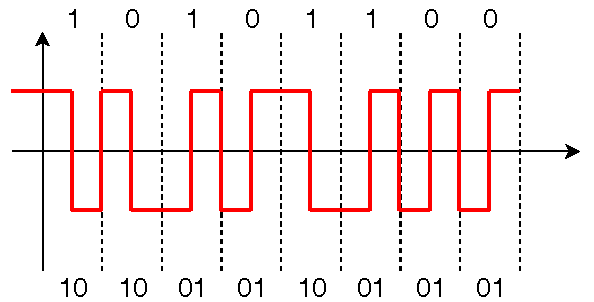
\includegraphics[width=0.5\linewidth]{fig/network-manchester.pdf}
\end{figure}
\item 4B/5B编码:用5比特代表4比特,多一位冗余;每个编码没有多于1个前导零和多于2个末端零,即\textemph{最多3个0};
防止跳变过多,又可消除基线漂移和时钟漂移
\begin{center}
\begin{tabular}{|c|c||c|c|}\hline
4B & 5B & 4B & 5B\\\hline\hline
0000 & 11110 & 1000 & 10010\\\hline
0001 & 01001 & 1001 & 10011\\\hline
0010 & 10100 & 1010 & 10110\\\hline
0011 & 10101 & 1011 & 10111\\\hline
0100 & 01010 & 1100 & 11010\\\hline
0101 & 01011 & 1101 & 11011\\\hline
0110 & 01110 & 1110 & 11100\\\hline
0111 & 01111 & 1111 & 11101\\\hline
\end{tabular}
\end{center}
\end{enumerate}

\subsection{物理介质}
\subsubsection{分类}
\begin{enumerate}
\item 有线介质
\begin{itemize}
	\item 双绞线:
	\begin{itemize}
		\item 非屏蔽双绞线(unshielded twisted pair, UTP):四对线(绿绿白、橙橙白、蓝蓝白、棕棕白),cat5/cat5e百兆以太网,cat6千兆以太网\footnote{1KB(Kilobyte,千字节),1MB(Megabyte,兆字节,简称``兆''),1GB(Gigabyte,吉字节,又称``千兆'')}
		\item 屏蔽双绞线(STP)
	\end{itemize}
	\item 同轴电缆(coaxial cable)
	\item 光导纤维(optical fiber):利用光的全反射性质
	\begin{itemize}
		\item 单模光纤(single mode):最大传输速率
		\item 多模光纤:阶跃(step-index)光纤、渐变(graded-index)光纤
	\end{itemize}
\end{itemize}
\item 无线介质:地面微波、WiFi、3G网络、卫星
\end{enumerate}

\subsubsection{多路复用方式}
\begin{itemize}
	\item 时分多路复用(time division multiplexing, TDM):时间域被分成周期循环的一些小段,每段时间长度是\textemph{相同}的,每个时段用来传输一个子信道
	\item 频分多路复用(frequency, FDM):\textemph{无线电台}常用
	\item 波分多路复用(wavelength, WDM):利用多个激光器在单条光纤上同时发送多束\textemph{不同波长}激光的技术
	\item 码分多路复用(code, CDM):利用各路信号码型结构正交性而实现多路复用
	\item 统计多路复用(static, SDM):\textemph{动态分配}方法共享通信链路,比如FIFO;对于多个\textemph{可变速率}的数据流,SDM可以提高链路利用率
\end{itemize}

% \begin{example}
% 	如果有8个速率相同的数据流,且它们速率之和小于且接近一条链路的带宽,与用8个通道(channel)的TDM或FDM传送它们相比,采用统计多路复用技术的带宽利用率(传送有效数据的比率)怎么样?
% \end{example}
% \begin{analysis}
% 	更差,都可以用完整个带宽,只是统计复用技术需要地址,因此会差一点
% \end{analysis}
% !TEX root = main.tex

\section{数据链路层}
数据链路层把数据包,即\textbf{帧(frame)},从一个节点通过链路(直连网络或\textbf{物理网络})传给相邻另一个节点(主机和路由器)。

数据链路层的功能如下:
\begin{itemize}
	\item 成帧(framing)
	\item 差错检测(error detect):比特错,纠错
	\item 差错控制(error control):丢包、重复、错序、流控制(flow control)
	\item 介质访问控制(medium access control):多路访问,碰撞(collision)
\end{itemize}

针对点对点和多路访问网络分别制定了两个子层:
\begin{itemize}
	\item 逻辑链路控制(Logic Link Control, LLC)子层:提供可靠数据传输
	\begin{itemize}
		\item LLC1提供\textbf{无确认无连接}服务
		\item LLC2提供\textbf{有确认面向连接}的服务,实现滑动窗口协议
		\item LLC3提供\textbf{有确认无连接}的服务
	\end{itemize}
	\item 介质访问控制(Media Access Control, MAC)子层:专门用来处理多路访问网络中的冲突(点对点网络没有冲突就不用)
\end{itemize}

注意数据链路层、网络层错了就错了,不提供纠正服务,由上层纠正。
链路层在网络接口卡(network interface card, NIC)及其驱动程序上实现,路由器在接口模块上实现。

\begin{figure}[H]
	\centering
	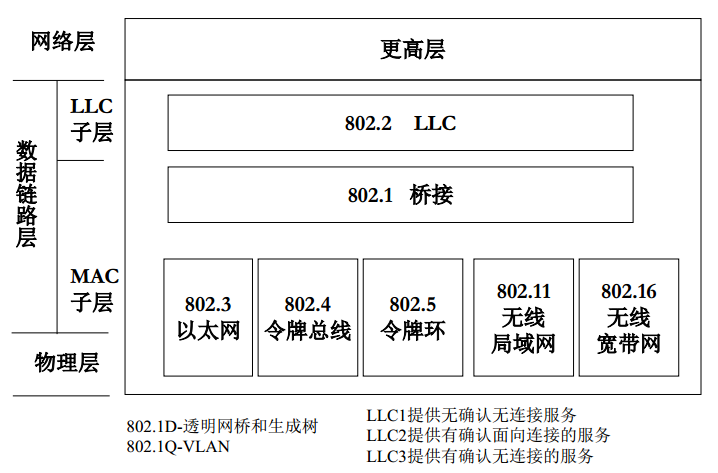
\includegraphics[width=0.6\linewidth]{fig/ieee802.PNG}
	\caption*{IEEE802系列标准}
\end{figure}

\subsection{逻辑链路控制子层}
\subsubsection{差错检测}
在数据报后加校验码(头部加序号),通过链路传输看是否有数据报/校验码错误。
\begin{enumerate}
\item 奇偶校验:若接收方收到奇数个1,则有出错
\begin{itemize}
	\item 一维偶校验:只能检错;最后补一位使得全部为偶数个1,如$010$补为$010\mid 1$,而$101$补为$101\mid 0$
	\item 二维偶校验:检错+纠错一位;横纵同时偶校验
\end{itemize}
\item 校验和(checksum):将所有数据加起来,每16位1组,最高位进位则\textbf{末尾加1},最后结果\textbf{取反}\\
由于需要使用加法器,校验和一般不用于数据链路层,而用在更高层,例如网络层和传输层
\begin{figure}[H]
	\centering
	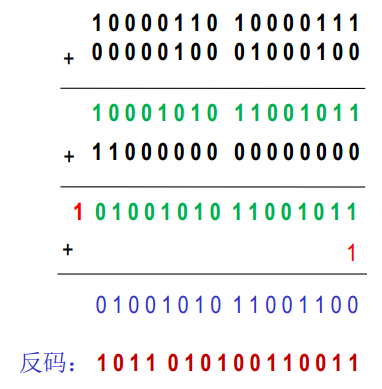
\includegraphics[width=0.4\linewidth]{fig/checksum.PNG}
\end{figure}
\item 循环冗余校验码(Cyclic Redundancy Check, CRC):
补充n位后除以一个n+1位的除数,模2除法(按位异或,做减法时没有借位)\\
接收方连带校验码一起除,余数为0则没错\\
如下图,4位除数补3个0,最后的余数011即为校验码
\begin{figure}[H]
	\centering
	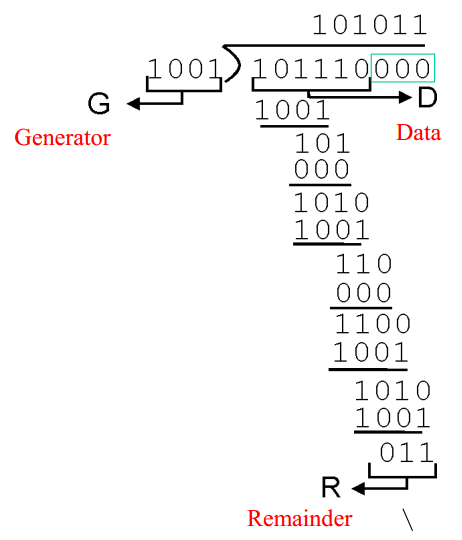
\includegraphics[width=0.4\linewidth]{fig/CRC.PNG}
\end{figure}
链路层常用CRC,因为检错率很高,且容易实现(触发器+异或门)
\end{enumerate}

\subsubsection{可靠数据传输}
每发送一帧都启动一个超时定时器,如果它的确认帧(Acknowledgement frame, ACK)在其超时时间内到达就删除该定时器;否则,自动重发请求(Automatic Repeat reQuest, ARQ)/重传该帧并重启定时器

主要的ARQ协议如下:
\begin{itemize}
	\item 停等协议(stop-and-wait):只有收到前一个数据帧的确认帧才可以发送下一个数据帧;最少需要2个序号。三种出错情况:
	\begin{itemize}
		\item 数据帧丢失(loss):正向传递时丢包
		\item 确认帧丢失:回传时丢包
		\item 超时:收到ACK表明接收方一定收到,可以发送新的数据帧,重传的也一定要发ACK
	\end{itemize}
	效率/吞吐量十分低,信道空闲时间长
	\item 滑动窗口协议(sliding window):不需等待前面发送的帧的确认帧返回,就可以连续发送下一个,其个数不能超过发送窗口大小(sending window size, SWS)\footnote{连续发送数据帧可用序号范围,用于流控制:控制发送速度,否则会发生溢出(overlow),后面覆盖前面的}\\
	这里的确认帧是指在此之前的帧都已全部收到并已交给上层协议(直连网中间没有节点,后面收到前面一定收到;只要出错纠正不了直接丢弃),后面确认前面,提高可靠性
	\begin{itemize}
	\item 回退N协议(go back N):同滑动窗口连续发送,某个ACK没收到则重传在此ACK之后的所有帧(超时重传),丢3则ACK4发2
	\begin{itemize}
		\item 发送窗口需要缓存SWS个帧,以便重传;发送窗口中序号最小的为sendbase
		\item 回退N协议可能会收到落在\textbf{发送窗口之外的确认帧},如果因确认帧迟到而出现超时重传,就可能收到一个帧的两个确认帧,第二个确认帧就会落在发送窗口之外
	\end{itemize}
	\item 选择性重传(selective repeat):通过发送否定性确认帧(negative acknowledgement, NAK)要求重传该帧;如3丢失,4发送NAK=3,5发送ACK=2,重传3
	\begin{itemize}
		\item 接收窗口(receiving window size, RWS)表示接收缓冲区大小(RWS$\leq$SWS,最好是等于,尽量减少重传帧;但序号少的话导致重复;错序到达的帧加上期待接收的帧最多SWS个),用于确定应该保存哪些帧,用序号范围表示
		\item 超时时间应该设长,确保帧的2次来回;没有后续帧也会超时重传;无论窗口内窗口外收到都要发确认
		\item 选择性重传协议可能会收到落在\textbf{接收窗口之外的数据帧},因确认帧丢失或超时到达而重传的数据帧都会落在接收窗口之外
		\item 选择性重传协议丢失了NAK并非致命错误,因为还有超时重传机制,保证该数据帧能够重新发送
	\end{itemize}
	\end{itemize}
\end{itemize}
\par ARQ协议的超时时间不应设置得太长,否则会导致系统需要花很长的时间来纠正这些错误;ARQ设得短可以使查出错误的时间变短,同时提升网络的吞吐量(但也不能设太短,否则发送方会大量误认为帧丢失而产生不必要重传)。

% 如果当前RTT=1ms,采用选择性重传(selective repeat)滑动窗口协议,超时时间应设置为略大于2ms;如果收到NAK就重置所有的超时定时器,那超时时间应设置为略大于1ms。
% 这里假设收到NAK的重传不重置超时定时器,否则,一个RTT也可以。

注意不管哪一种重传机制,序号可以重复使用,因此有最小序号问题。
\begin{example}
	序号8个,SWS=RWS=4,345670123456,5丢失
\end{example}
\begin{analysis}
	回退N:346705670123456\\
	选择性重传:346705123456
\end{analysis}
\begin{example}
	把停等协议用于一个带宽为20Mbps、长度为3000公里、传播速度为200000公里/秒的点到点链路,如果最长帧为5000字节,带宽的最大利用率(最大吞吐量/带宽)是百分之多少?
\end{example}
\begin{analysis}
	按照如下方法计算
	\begin{itemize}
		\item 传播延迟$RTT$:$(3\times 10^6 m) / (2\times 10^8 m/s)\times 2=30ms$(注意是\textbf{往返时间}!)
		\item 传输延迟$L/R$:$(5000B\times 8)/(20\times 10^6bps)=2ms$
		\item 吞吐量:$L/(RTT+L/R)=(5000B\times 8)/32ms=1.25Mbps$
		\item 带宽最大利用率:最大吞吐量/带宽=$1.25/20\times 100\%=6.25\%$
	\end{itemize}
	另,改为滑动窗口协议,窗口大小为8,则最大利用率位$8\times 6.25\%=50\%$
\end{analysis}

提高滑动窗口协议的效率:
\begin{itemize}
	\item 选择性确认(selective acknowledgement):接受方把已收到的帧的序号告诉发送方(收到不用重传告诉发送方哪些已收到,则只用重传某帧)
	\item 捎带确认(piggybacking):通信双方\textbf{全双工}方式工作,接收方在发数据给对方时顺便把确认号也告诉对方(两个滑动窗口,两边都要发数据),需要结合下面一起使用
	\item 延迟确认(delayed acknowledgement):接收方收到一帧后并不立即发送确认帧,而是等待一段时间再发送
\end{itemize}

\subsection{介质访问控制子层}
\subsubsection{简介}
\begin{enumerate}
\item \textbf{PPP协议(point-to-point):点对点网络}
\begin{itemize}
	\item 根据HDLC(high-level data link control)协议进行设计,主要用于串行电缆、电话线(MODEM)等串行链路
	\item 提供连接认证、传输加密和压缩功能,为网络层协议提供服务
	\item 采用字节填充法(byte-stuffing)替换掉保留字
	\item 没有纠错功能,也没有流控制和确保有序的功能
	\begin{figure}[H]
		\centering
		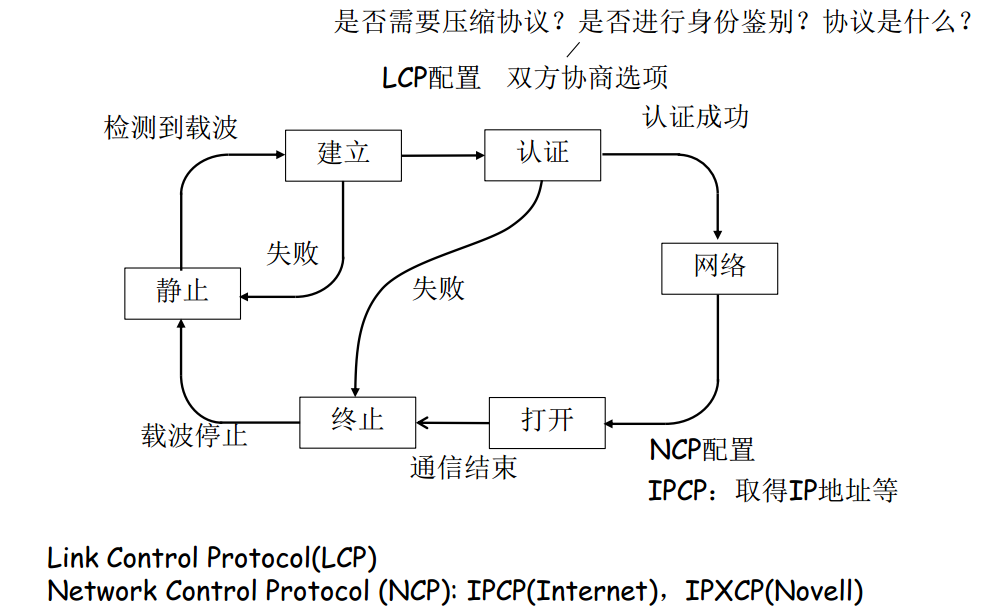
\includegraphics[width=0.6\linewidth]{fig/PPP.PNG}
	\end{figure}
\end{itemize}

\item \textbf{以太网:多路访问网络}\\
解决冲突问题:随机访问协议(random access protocol),注意不是滑动窗口不用发确认帧
\begin{itemize}
\item 纯ALOHA:想发送就发送,超时未收到确认则发生冲突
\item 分槽ALOHA:将时间分为长度相同的时槽,每个站点只在时槽开始时发送。\\
信道空,立即以概率$p$发送,以概率$1-p$延迟一个时间槽;信道忙,延迟一个时间槽。
\item 载波监听CSMA(Carrier Sense Multiple Access):发送前先监听信道
\begin{itemize}
	\item 信道空,立即发送;信道忙,持续监听(1-persistent CSMA,以太网)
	\item 信道空,发送;信道忙,延迟一段随机长度时间(non-persistent CSMA),较省电
	\item 信道空,立即以概率$p$发送,以概率$1-p$延迟一个时间槽;信道忙,延迟一个时间槽(p-persistent CSMA,分槽ALOHA)
\end{itemize}
\end{itemize}
\end{enumerate}

\subsubsection{以太网物理层协议}
IEEE 802.3规定以太网物理层标准:
\begin{itemize}
	\item 传输方法:均使用\textbf{异步传输},即信道空闲时以太网设备不任何发送信号
	\item 编码方法:曼彻斯特编码
	\item 命名规则: 10BaseT的10表示10Mbps,Base表示基带传输,T表示双绞线;10base2的2表示最大距离200m
\end{itemize}
与802.3相比,快速以太网(100BaseTX)只是把传输速率提高到100Mbps
\begin{itemize}
	\item MAC子层的协议不变:CSMA/CD协议不变,帧格式不变
	\item 最大距离改为100m (10base5的最大距离为2500m),物理层改动
	\item 帧间空隙隔依然为96b,即$0.96\mu s$
\end{itemize}

集线器(hub)采用电子线路方法模拟总线方式的以太网,两台主机同时发送会产生冲突,所以是\textbf{半双工}工作。
如果通过两个接口同时发送数据会产生冲突,则这两个接口属于同一个冲突域(collision domain)。一个广播帧可以到达的所有接口属于同一个广播域。
属于同一个冲突域的以太网部分称为网段(segment)。
\begin{example}
	下图的冲突域和广播域个数?
	\begin{figure}
		\centering
		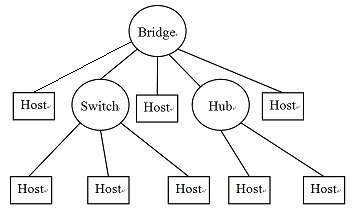
\includegraphics[width=0.35\linewidth]{fig/conflict_count.jpg}
	\end{figure}
\end{example}
\begin{analysis}
交换机(switch)/网桥(bridge)的每个端口处于一个冲突域,集线器(hub)的所有端口处于一个冲突域。故8个冲突域,1个广播域。
\end{analysis}

集线器、交换机、路由器区别见\ref{subsub:physical_equipment}节。

\subsubsection{以太网MAC层协议}
以太网采用帧间空隙(interframe space)的成帧方法(每帧发送前要求信道空闲时间至少为96bits,造成每帧之间有空隙)。
采用载波监听CSMA/CD(with collision detection)协议(1-坚持CSMA)。
\begin{enumerate}
	\item 发送数据帧之前先监听信道。如果信道空闲,\textbf{立即}发送。
	如果信道忙,则\textbf{持续监听},直到信道空闲,立即发送。
	\item \textbf{边发送边检测}冲突。如果发送完毕都没有检测到冲突,则发送成功。
	\item 如果检测到冲突,则\textbf{停止发送},并发送32位干扰位(jamming signal)以加强冲突信号。
	采用二进制指数退避算法\textbf{随机延迟}一段时间后,转(1)。
\end{enumerate}

二进制指数退避算法(binary exponential backoff)
\begin{itemize}
	\item 规定最短帧是为了使发送站点可以监测到所有冲突,选择最短帧的发送时间作为其时间槽(time slot)$\tau$的长度,最短帧的发送时间保证了首先发送的站点的信号可以到达最远的站点。如果先发送的只有一个站点,其他站点要不就检测到发送站点的信号而不能发送,要不就因为发送站点发送完毕而检测到信道空闲,总之不会与之冲突。也就是说,任何间隔$\tau$或以上时间的两个发送数据的站点不会发生冲突。
	\item 时间片$\tau$的长度为512b时间,10Mbps的以太网为51.2$\mu s$
	\item 第$i$次冲突从$0,1,\ldots,2j-1$个时间片随机选择一个,$i<16$,$j = min(i,10)$
	\item 前十次冲突后可选时间片数量每次加倍,后五次冲突后可选时间片数量不变,所以也称	为截止式(truncated)二进制指数退避算法
\end{itemize}
\begin{example}
	当一个以太网的信道忙时有五个站点都想发送一个最长帧(长度为1520B),如果很长时间只有这五帧要发送,问最少经过几次冲突就可以全部发送成功?
\end{example}
\begin{analysis}
	最长帧占用$1520B\times 8/512b=23.75$个时间槽,而在第1、2、3、4次冲突的延迟时间最多16个时间槽,首先发送的站点都会引起后续所有站点冲突。
	最好情况每次冲突后都让一个站点发送成功,所以最少4次冲突。
	详细来说,一开始5个站点同时发送,第一次冲突,随机延迟0或1个时间片,假设0号立即发送,其他4个延后1个时间片,那么0号发送成功,其他4个检测到信道忙,不发送。
	到0号发完时,信道空闲,其他4个同时发送,第二次冲突,如此类推,每次成功发送一个。
\end{analysis}

802.3的MAC帧格式
\begin{center}
前导字符(8B)+目的地址(6B)+源地址(6B)+类型/长度(2B)+有效载荷/填充位+帧校验序列(4B)
\end{center}
\begin{itemize}
\item 源地址:一般为发送者的单播地址
\item 目的地址(6B):一般为接收者的单播地址
\end{itemize}

MAC地址
\begin{itemize}
	\item 单播/网卡/烧录地址:全球唯一,每个网卡/接口一个
	\item 多播地址:字节0第0位为1,地址非全1
	\item 广播地址:48位全为1
\end{itemize}

\subsubsection{透明网桥}
透明网桥的三个操作:
\begin{itemize}
	\item 表里查到则\textbf{转发}(forward)
	\item 表里没有则扩散/\textbf{泛洪}(flood):由端口P1,扩散到其他所有端口P2,P3(多播、广播一定扩散)
	扩散不回传
	% 只要广播都要收下了,操作系统一定要处理
	收到的部分不会往回转
	\item 从某一条路发来则不能传回去,过滤/\textbf{丢弃}(filter)
\end{itemize}

透明网桥有自学习机制:利用\textbf{源地址}学习,如信息从A主机-P1端口来,则记为A-P1,同时设好生存期(Time to live, TTL)\footnote{单位为秒,每次发送都会重置,对于不活跃的表项自动删掉(减少表的大小,查找速度更快)}。
如果收到的帧有错则直接丢弃,根本不会学习。
如果源地址已经在表中,则更新记录,并重置超时计时器。

扩展/桥接局域网:每一个局域网(LAN)都是一个网段
\begin{example}
	下面的扩展LAN包含三个透明网桥B1、B2、B3和四台主机A、C、D、E。
	如果网桥的MAC地址表初始都是空的,在以下三次传输之后MAC地址表的内容是什么?
	\begin{enumerate}
	\item D发送了一个帧给E
	\item A发送了一个帧给D
	\item C发送了一个帧给A
	\end{enumerate}
	\begin{figure}[H]
		\centering
		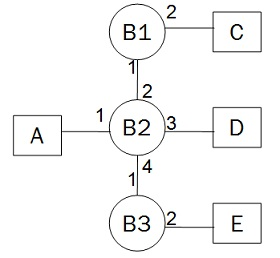
\includegraphics[width=0.3\linewidth]{fig/mac_address.jpg}
	\end{figure}
\end{example}
\begin{analysis}
	\begin{minipage}{0.32\linewidth}
	\begin{table}[H]
		\centering
		\caption*{B1的MAC地址表}
		\begin{tabular}{|c|c|}\hline
			MAC地址 & 端口 \\\hline
			D & 1\\\hline
			C & 2\\\hline
		\end{tabular}
	\end{table}
	\end{minipage}
	\begin{minipage}{0.32\linewidth}
	\begin{table}[H]
		\centering
		\caption*{B2的MAC地址表}
		\begin{tabular}{|c|c|}\hline
			MAC地址 & 端口 \\\hline
			D & 3\\\hline
			A & 1\\\hline
			C & 2\\\hline
		\end{tabular}
	\end{table}
	\end{minipage}
	\begin{minipage}{0.32\linewidth}
	\begin{table}[H]
		\centering
		\caption*{B3的MAC地址表}
		\begin{tabular}{|c|c|}\hline
			MAC地址 & 端口 \\\hline
			D & 1\\\hline
		\end{tabular}
	\end{table}
	\end{minipage}
\end{analysis}

之所以称为透明,是因为插入网桥后无需改动硬件和软件,也无需设置地址开关、装入路由表或参数等,网桥就能工作(自学习)。

\subsubsection{生成树协议}
将所有的LAN和网桥都抽象为结点,避免冲突即构造一棵生成树(注意不是最小生成树)
\begin{itemize}
\item IEEE 802.1D 生成树协议+透明网桥
\item IEEE 802.1w RSTP(Rapid Spanning Tree Protocol)
\end{itemize}

工作流程如下
\begin{itemize}
\item 先确定根网桥,即\textbf{BID(Bridge ID)最小}的
\item 每个网段(需要集线器)依赖于连通的网桥,每个网桥都把自己到根的距离发出去(竞选/配置消息)
\item 网桥之间的开销为1,选一条\textbf{最短路径}
\item 扩散自己BID,最后只剩下根网桥认为自己是根
取得优胜的,作为指定网桥;相同距离时,BID小的优胜;端口号小的优胜
\item 网桥只在根端口和指定端口之间转发\textbf{数据}帧,不可通过阻塞端口
\item 只有从根端口过来的才扩散配置消息,其他端口来的不扩散,这样不会形成回路
\item 断了/失效了则变成无穷大,其他网桥可成为指定网桥
\end{itemize}

防止广播风暴,又能自动修复损害网桥(通过冗余方式),增加可靠性
\begin{example}
	下图显示了由五个透明网桥(B1~B5)形成的扩展LAN。
	\begin{figure}[H]
		\centering
		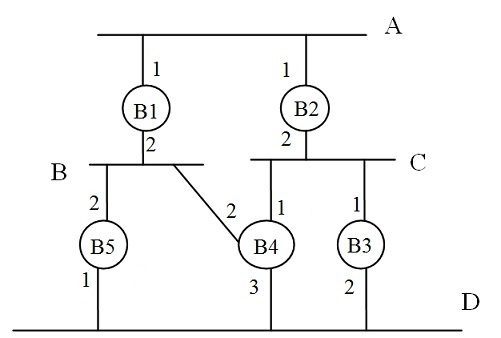
\includegraphics[width=0.4\linewidth]{fig/bridge.jpg}
	\end{figure}
\end{example}
\begin{analysis}
\begin{enumerate}
	\item B1是根网桥
	\item 网段A-D的指定网桥(designated bridges)分别是
\begin{center}
	\begin{tabular}{|c|c|c|c|}\hline
		A & B & C & D\\\hline
		B1 & B1 & B2 & B4\\\hline
	\end{tabular}
\end{center}
\item 网桥B1-B5的根端口分别是
\begin{center}
	\begin{tabular}{|c|c|c|c|c|}\hline
		B1 & B2 & B3 & B4 & B5\\\hline
		无 & 1 & 1 & 2 & 2\\\hline
	\end{tabular}
\end{center}
\end{enumerate}
\end{analysis}

\begin{example}
	下图是一个扩展LAN:
	\begin{figure}[H]
		\centering
		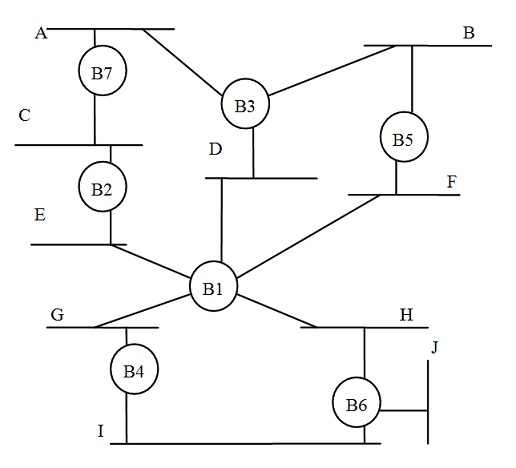
\includegraphics[width=0.4\linewidth]{fig/spanning_tree.jpg}
	\end{figure}
\end{example}
\begin{analysis}
	\begin{itemize}
		\item[a.] 如果B1没有启动生成树算法但是转发生成树消息(BPDU),只生成1棵生成树,根为B2
		\item[b.] 如果B1没有启动生成树算法而且丢弃所有收到的生成树消息(BPDU),生成2棵生成树,根分别为B2和B4
	\end{itemize}
\end{analysis}

\subsubsection{虚拟局域网}
虚拟局域网(Virtual LAN, VLAN)将原来的局域网分割成多个相互隔离的局域网,只在具有相同颜色的端口间转发。

如果所有交换机都是连通的,并且交换机连至交换机的接口都配置为trunk接口,交换机连至主机的接口都配置为VLAN接口(主机接口),则所有连至相同的VLAN接口的主机都位于同一个广播域,连至不同VLAN接口的主机位于不同的广播域。

每次扩散扩散到帧内指定的端口或\textbf{干道端口},同样查MAC地址表转发。
只有发往干道端口的帧才需要加上VLAN ID。
如果从干道收到的帧没有VLAN ID,则认为是本征(native)VLAN,默认为VLAN1。
\begin{example}
	下图中哪些发送的帧将被目的主机收到
	\begin{figure}[H]
		\centering
		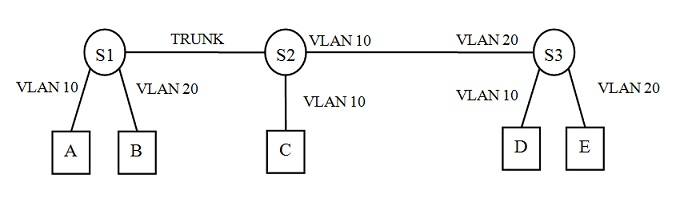
\includegraphics[width=0.5\linewidth]{fig/vlan.jpg}
	\end{figure}
\end{example}
\begin{analysis}
	只有A到E或E到A可以成功发送信息,注意S2和S3的端口设错了(故意的)。
	如E到A,VLAN20经过S3转发到VLAN20,发到S2。
	S2误认为是从VLAN10发来的消息,故扩散到干道端口TRUNK加VLAN10,发到S1。
	S1接收到后转发至VLAN10。\\
	而D到B没有办法,因为从S3就转发不出去,没有干道端口。
\end{analysis}

多生成树协议:管理员规定哪些VLAN为一组,构成多生成树,其余的用公共生成树
\begin{itemize}
	\item 公共生成树(common spanning tree, CST)
	\item 多生成树(Multiple spanning tree protocol, MSTP)
\end{itemize}

\subsubsection{令牌环网}
令牌环网(token ring):通过在站点之间传递令牌防止冲突并且具有
\textbf{优先权}的星形\textbf{LAN},其标准为IEEE 802.5,take turns protocol,现在有千兆令牌环网。
多站点接入部件称为(multistation access unit, MSAU)
\begin{figure}[H]
	\centering
	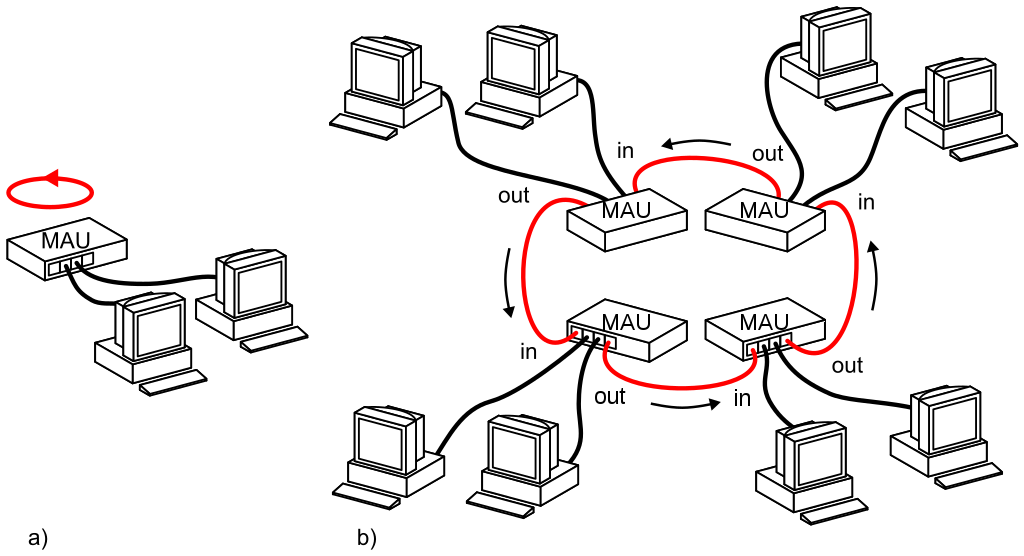
\includegraphics[width=0.5\linewidth]{fig/token-ring.png}
\end{figure}

数据传送过程:
\begin{itemize}
	\item 令牌(帧)绕环而行
	\item 只有截获令牌的站点才可以发送数据帧,各站点保有令牌帧的时间是相同的
	\item 发送的数据帧通过所有的活动站点
	\item 目的站点拷贝数据帧
	\item 只有发送方移除数据帧
	\item 当没有数据帧要发送或者持有时间到,当前的发送站点要释放令牌;被释放的令牌继续绕环而行
\end{itemize}

注意:以太网没有确认机制,没有优先权。
必然有特殊的站点(监控站点)产生令牌帧,选举出监控站点(MAC地址最小)。

源路由桥接算法:由IBM开发的用于令牌环网的协议,将路径记到头部,下一次就不用查。
为了兼容普通交换机,源路由网桥交换机也必须实现透明网桥的功能。

\subsubsection{物理设备}
\label{subsub:physical_equipment}
交换机是一个把多个网段连接起来的设备,也称为\textbf{多端口网桥}(switch=bridge)。
注意输入输出端口一样。

交换结构(fabrics)
\begin{itemize}
	\item 共享总线式交换机:同样有冲突问题
	\item 纵横式(crossbar):可实现多路并行传输
\end{itemize}

交换机转发方法
\begin{itemize}
\item 存储转发(store and forward):交换机收到整个帧后转发\\
目的MAC地址(6B),转也要依照CSMA/CD来转发
\item 直通(cut through):收到一个转一个,出现碎片
\item 无碎片(fragment free):都没冲突才开始转发,\textbf{最小帧保证}\\
交换机不用收到整个帧而是收到64B(冲突窗口)后自动转发
\item 适应性交换(adaptive switching):自动在上面三种方式中选择
\end{itemize}

交换机的工作模式
\begin{itemize}
\item 全双工模式:因为没有冲突,CSMA/CD算法可以被关闭
\item 自动翻转(auto-MDIX):
大部分交换机可以自动选择连接方式,\textbf{交叉线}或\textbf{直通线}
\item 自适应(autonegotiation):两个站点周期性使用快速链路脉冲(fast link pulse,FLP)选择10M/100M/1000Mbps自适应
\end{itemize}

% 如果主机A发送IP分组给主机B, 主机B收到的帧中的源地址是什么?
% 连接模式: [host A]--[Router R1]--[Router R2]--[host B],其中包含3个以太网。
% R2的MAC地址

集线器、交换机、路由器的区别如下\footnote{\url{http://www.qianjia.com/html/2017-08/09_274208.html}}:
\begin{itemize}
	\item 集线器(hub):\textbf{物理层/一层},广播,排队,冲突,共享型设备(一个端口往另一个端口发数据,其他端口就处于等待状态,全部端口属于一个冲突域),半双工,监听,响应
	\item 交换机(switch):\textbf{数据链路层/二层},MAC地址,建立连接,独享信道,全双工,增加冲突域数量,减少冲突范围大小
	\item 路由器(router):\textbf{网络层/三层},建立路由表,IP地址,路由选择
\end{itemize}

路由器与其他两者的区别:
\begin{enumerate}
\item 集线器工作在第一层,没有智能处理能力,对它来说,数据只是电流,当一个端口的电流传到集线器中时,它只是简单地将电流传送到其他端口,至于其他端口连接的计算机接收不接收这些数据,它就不管了。
交换机工作在第二层,它要比集线器智能一些,对它来说,网络上的数据就是MAC地址的集合,它能分辨出帧中的源MAC地址和目的MAC地址,因此可以在任意两个端口间建立联系,但是交换机并不懂得IP地址,它只知道MAC地址。
路由器工作在第三层,它比交换机还要更智能一些,它能理解数据中的IP地址,如果它接收到一个数据包,就检查其中的IP地址,如果目标地址是本地网络的就不理会,如果是其他网络的,就将数据包转发出本地网络。

\item 路由器能连接不同类型的网络,我们常见的集线器和交换机一般都是用于连接以太网的,但是如果将两种网络类型连接起来,比如以太网与ATM网,集线器和交换机就派不上用场了。
路由器能够连接不同类型的局域网和广域网,如以太网、ATM网、FDDI网、令牌环网等。
不同类型的网络,其传送的数据单元---帧的格式和大小是不同的,数据从一种类型的网络传输至另一种类型的网络,必须进行帧格式转换。
路由器就有这种能力,而交换机和集线器就没有。
而互联网就是由各种路由器连接起来的,因为互联网上存在各种不同类型的网络,集线器和交换机根本不能胜任这个任务,所以必须由路由器来担当这个角色。

\item 路由器具有路径选择能力,在互联网中,从一个节点到另一个节点,可能有许多路径,路由器可以选择通畅快捷的近路,会大大提高通信速度,减轻网络系统通信负荷,节约网络系统资源,这是集线器和二层交换机所根本不具备的性能。
\end{enumerate}

小范围的局域网,如我们的校园网大多采用交换机,路由少。

注意交换机\textbf{相当于\textcolor{red}{透明}网桥},故路由器不会知道,路由器只知道下一跳。
% !TEX root = main.tex

\section{网络层}
\subsection{IP数据报}
\subsubsection{数据传输技术}
\begin{itemize}
\item 电路交换(circuit switching):实际接通一条物理线路,时分多路复用,电话;频分多路复用,电视;一直占用,不管有无数据交互
\item 包交换/分组交换(packet switching):统计多路复用,按需分配;可能引起网络拥塞,适合发送突发数据
\begin{itemize}
	\item 虚电路:需建立连接才可以传输数据(仿照电话系统,因特网之前),好处在于保留带宽
	\begin{itemize}
	    \item 交换式(要交换才建立连接):建立虚电路(VC)表,虚电路标识符(VCI),类似于电话
	    \item 永久式(建立后一直保持):由管理员维护
	\end{itemize}
	\item 数据报(datagram):不需建立连接,因特网,\textbf{不预留带宽}
\end{itemize}
\end{itemize}

一般网络的服务模型:Aynchronous Transfer Mode, ATM
\begin{center}
\begin{tabular}{|c|c|c|c|c|c|c|}\hline
网络结构 & 服务模型 & 带宽 & 不丢包 & 有序 & 及时 & 拥塞反馈\\\hline
ATM & 恒定位速率 & 固定速率 & 是 & 是 & 是 & 无拥塞\\\hline
ATM & 可变位速率 & 确保速率 & 是 & 是 & 是 & 无拥塞\\\hline
ATM & 可用位速率 & 最小保证 & 否 & 是 & 否 & 是\\\hline
ATM & 未指定位速率 & 无 & 否 & 是 & 否 & 否\\\hline
因特网 & 尽力服务 & 无 & 否 & 否 & 否 & 否\\\hline
\end{tabular}
\end{center}

IP协议是因特网的网络层协议
\begin{itemize}
\item 可路由的(routable):全局地址,按层分配
\item 尽力服务(best effort):无连接无确认的数据报服务
\item IP协议可以运行在\textbf{任何}网络上,不仅仅是因特网
\end{itemize}

\subsubsection{IP数据报格式}
\begin{itemize}
\item 4个字节一个字,头部最多$(2^4-1)*4=60$B,除选项20B,IPv4选项最多40B,太少了
\item 生存期(TTL)限制在因特网上的停留时间,实际限制为经过的路由器数目,即跳数(hop count),超过则自动清除,防止兜圈,每次经过路由器减1\\
TTL初值默认设置为网络直径的两倍,Windows默认64\\
长了就有捷径(cut-through),因此发展到现在因特网的直径依然在32左右
\item IP数据报一定要封装成帧,通过物理层传输,每次都要修改源和目的地址
\item IP数据报服务类型(type of quality, ToQ),但路由器都没有实现
\end{itemize}

IP数据报的分段和重组
\begin{itemize}
\item 一个物理网络的最大传输单元(maximum transmission unit, MTU)是该网络可以运载的最大有效载荷,即数据帧的数据部分的最大长度\\
如:以太网(DIXv2)的MTU为1500, FDDI和令牌环的MTU分别为4353和4482
\item 只要发出去一定会封装成帧(注意要加头部),帧最长就是MTU,因而要分成多段再分
\item 如果一个数据报的大小大于要承载它的网络的MTU,路由器需要先对该数据报进行分段(fragment)
\item 源主机每次发送IP数据报时都会把标识(Identification)字段加1。
\item 分段时用标识的值保持不变,并且用偏移量字段(offset)指出该片段的数据部分相对原来数据报的偏移量(以8字节为单位),给出原来片段的次序
\item MF(More Fragment), DF(Don't Fragment)
\item 小于MTU-20B,边界,一定要能被8整除,尽可能大(8字节,一定要除掉)
\item IPv6中间不能分段
\item 1400B=512B+512B+376B
\item Path MTU discovery:找到路径上最小的MTU,发现路径上最小MTU
\item 选项最后一定对齐到边界
\item 生存期和头部校验(检验和)会变,其他不变
\end{itemize}

\subsection{IP地址}
48位的MAC地址和32位的IP地址都是全局的(全球分配),但是IP地址空间分层,是可路由的

IP地址可划分为两个部分:
\begin{itemize}
	\item 网络号/网络前缀/网络标识:确定拥有该IP地址的主机位于哪个网络
	\item 主机号:确定属于该网络的哪台主机
\end{itemize}

有类网:ABC单播,D多播,E保留,地址范围如下(点分十进制)
\begin{itemize}
	\item 0 $\thicksim$ 127
	\item 128 $\thicksim$ 191
	\item 192 $\thicksim$ 223
	\item 224 $\thicksim$ 239
	\item 240 $\thicksim$ 255
\end{itemize}

解决IPv4地址不够用的问题
\begin{itemize}
	\item 将一个有类网可以划分为多个相同大小的子网(subnet)\\
用子网掩码(subnet mask)划分边界:主机号全0,剩下的部分(网络号和子网号)全是1\\
子网掩码与IP地址\textbf{相与},若相等则在同个子网中
	\item 变长子网掩码(Variable-length subnet mask, VLSM):允许把一个有类网划分为多个不同大小的子网,类似变长指令集\\
解决主机数目不均匀的问题,如100、50、25、10,则不能等距划分子网\\
用长度来表示子网掩码,如/26代表255.255.255.192
	\item 无类域间路由选择协议(classless inter-domain routing, CIDR):将多个有类网合并为一个更大的网络,称为超网(supernet)\\
可以显著减少路由表中路由的数量,称为路由聚合(route aggregation)
	\item 网络地址转换(network address translation, NAT):\textbf{最节约地址的方法},将内部地址映射为外部地址的技术(可以扩展6w多倍),将私有地址映射为全局地址\\
NAT将内部源地址转换为外部地址\\
NAPT将端口号也加入NAT的映射中
\end{itemize}

地址解析协议(address resolution protocol, ARP)可以\underline{将IP地址映射为MAC地址}\footnote{也有将也有MAC映射为IP地址的协议}
\begin{itemize}
	\item ARP请求广播帧(谁的IP地址是XXX),ARP响应单播帧(返回MAC地址),IP地址与MAC地址的端口号相同
	\item 没有超时重传机制,超时没有收到响应则丢弃引发ARP查询的IP分组
	\item 源主机获得的映射结果缓存在ARP表中$\lrang{\text{IP address},\text{MAC address},\text{TTL}}$,TTL一般为2到20分钟
	\item 当收到ARP请求,目的主机会缓存源主机的映射,其他主机如果已缓存该映射,则会重置TTL
	\item 也可直接将映射加入ARP缓存,称为静态ARP映射,不会因超时而删除
	\item 源硬件地址和协议地址、目标协议地址都知道,但\textbf{目的硬件地址}不知
\end{itemize}
\begin{figure}[H]
	\centering
	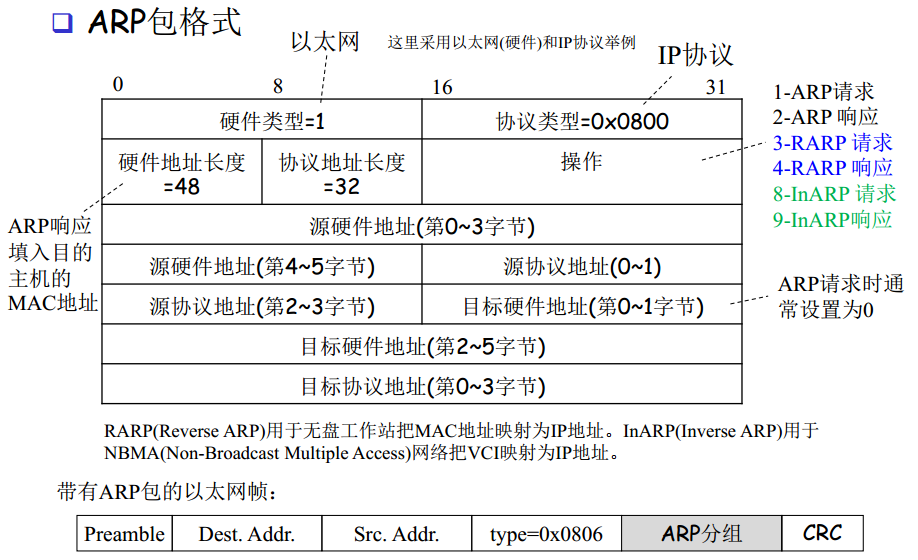
\includegraphics[width=0.7\linewidth]{fig/ARP.PNG}
\end{figure}

DHCP协议(Dynamic Host Configuration Protocol)用于主机在加入网络时\textbf{动态租用}IP地址,用UDP,四个步骤如下
\begin{itemize}
	\item DHCP发现(discover)
	\item DHCP提供(offer)
	\item DHCP请求(request)
	\item DHCP确认(ACK)
\end{itemize}

因特网控制消息协议(Internet Control Message Protocol, ICMP)用于主机或路由器发布网络级别的控制消息,主要是出错/丢包后将信息发回给源主机(TTL减到0、不可达),如回响请求和答复消息(ping)、不可达消息、时间超时消息(原IP头部+原IP数据部份的头64B)、重定位消息

% Path MTU Discovery 用于寻找路径上最小MTU
% Traceroute 用于获得整条路径上的路由器IP地址
% 交换机端口镜像Port Mirroring, also known as SPAN (Switched Port Analyzer) 实现监听
% DHCP Relay(中继) 多个局域网共享一个DHCP服务器 https://www.netmanias.com/en/post/blog/6004/dhcp-network-protocol/what-is-a-dhcp-relay-agent

\subsection{路由协议}
有类网的路由选择算法:
利用数据包中的\textbf{目的地址}得到\textbf{目的网络号},然后查询\textbf{路由表}(routing table)/转发表(forwarding table)
\begin{itemize}
	\item 如果查询的结果为\textbf{直连网},则\textbf{下一跳(next hop)为空},直接把数据包从查出的接口转发到目的主机
	\item 否则,如果查询得到\textbf{下一跳}(路由器),则把数据包转发给下一跳
	\item 如果没有查到任何匹配项,则把数据包转发给\textbf{默认路由器}(也算查到)
	\item 如果没有设置默认路由,则\textbf{丢弃}该数据包
\end{itemize}

无类网的路由选择:
无类网的路由表里有子网掩码
\begin{itemize}
	\item 匹配方法: 目的IP地址 \& 子网掩码 $==$ 子网号
	\item 最长匹配原则(The longest match rule): 当有多条路由都匹配时选择子网掩码最长(1的长度)的路由,因为更详细
	\item 从IP数据报中获取目的地址,利用目的地址\textbf{查路由表}(同有类网)
	\item 直连网将数据报直接\textbf{封装成帧}发送,不需要目的地址(PPP)
	\item 以太网同样要封装成帧,从\textbf{路由表中查出下一跳}的IP地址,通过\textbf{ARP协议}获得\textbf{目的MAC地址},加入帧内
	\item 如没有下一跳,则直接取\textbf{IP数据报中的目的IP地址}(已经到达了)
	\item 发送时要遵守以太网协议(CSMA/CD)
	\item 每到一个路由器都将帧拆出来,再重新封装,目的和源MAC地址(上一跳路由器MAC地址)全要发生变化
\end{itemize}

路由表
\begin{itemize}
	\item 127.0.0.1是内部的,其他是外部的需要经过防火墙
	\item 接口不一样,因此要在路由器里写两项,一项内部一项外部
	\item 往外发,默认路由会匹配
	\item 选择跃点数(metric)小的一项,如果跃点数也相同,则两个接口都会发送
\end{itemize}
% 点到点可以路由器端口不用配IP地址,但以太网一定要配,因为可能有交换机

路由表可以由管理员手工建立,也可以由路由/路由选择协议(routing protocols)自动建立。
路由协议即自动建立路由表,包括网络号、子网号、下一跳、接口、开销等。
所建立的路由分别称为\textbf{静态路由}和\textbf{动态路由}。
默认路由和直连路由都是静态路由。

建路由表是记\textbf{最短路径}的下一跳。

整个因特网实际上由很多机构进行管理。每个机构管理自己的网络,它们有权决定采用什么协议和网络控制策略。这样在\textbf{同一个机构}管理下的网络称为一个\textbf{自治系统}(autonomous systems, AS)。因特网实际上是由很多自治系统构成的。
\begin{itemize}
	\item 用于在AS\textbf{内部}(Intra-AS)建立动态路由的路由协议称为\textbf{内部网关协议}(Interior Gateway Protocols, IGP)。例如,\underline{RIP协议}和\underline{OSPF协议}。一个AS通常运行单一IGP。
	\item 用于在AS\textbf{之间}(Inter-AS)建立动态路由的路由协议称为\textbf{外部网关协议}(Exterior Gateway Protocol, EGP)。例如,\underline{BGP协议}。
	\item 运行同一个IGP协议的连通区域也称为路由选择域(routing domain)。一个AS可以运行多个IGP协议,形成多个路由选择域。
\end{itemize}

加了网关相当于加了默认路由。

网络层在入口位置有防火墙,未查路由表就丢弃了。

路由算法(Routing algorithm):路由协议里用的算法, 由于两个路由器之间都有开销,可以建立一个图,找最短路径
\begin{itemize}
	\item 链接状态(link state, LS):Dijstra
	\item 距离向量(distance vector, DV):BellmanFord
\end{itemize}

\subsection{内部网关协议}
\subsubsection{RIP协议}
路由信息协议(Route Information Protocol, RIP):\textbf{距离向量}算法的路由协议(问路),工作原理是\underline{采用邻居的路由表构造自己的路由表}。
\begin{itemize}
	\item 每\textbf{30秒}\footnote{太频繁会占用带宽}RIP路由器把它的整个路由表发送给邻居。具体实现时每个邻居会错开发送,30秒的时间也会随机变化一点。
	\item 初始时每个RIP路由器只有到直连网的路由,它们的距离为1。
	\item 到目的网络的距离以跳为单位。最大距离为15。距离16表示无穷大,即目的网络不可达。
\end{itemize}

具体算法:
当收到邻居发来的路由表(update packet),路由器将更新它的路由表$\lrang{\text{目的网络},\text{开销},\text{下一跳}}$:
\begin{enumerate}
	\item 收到路由的距离全部加1(即一跳的距离)
	\item 利用上述路由修改路由表:
	\begin{itemize}
		\item 把路由表中不存在的路由加入路由表
		\item 如果比路由表中的路由的距离更小,则更新该路由的距离为新距离,把下一跳改为邻居。如果原来的更大,则\textbf{也要进行改动},因为原来的路可能断了。即路由的下一跳送来的新路由,则必须修改距离。
	\end{itemize}
	\item 如果路由存在,就要重置失效定时器
\end{enumerate}
RIP路由表的每一项都有TTL(Time-To-Live),用失效定时器(invalid timer)计时,超时则让该路由失效

RIP协议存在的问题
\begin{itemize}
	\item 慢收敛:最短时间接近$0$(这样看更新时刻),最长时间$30(m-1)$,平均时间$15(m-1)$
	\item 计数到无穷:N1-R1通路断了,R1收到R2的路由表,更改自己的
\end{itemize}

RIP协议的技术
\begin{itemize}
	\item 水平分割(split horizon)技术:从一个接口学来的路由不会从该接口发回去;依然会计数到无穷,三角形R1断了,R1先发,R2后发
	\item 毒性反转(poison reverse)技术:当一条路由变为无效之后,路由器并不立即将它从路由表中删除,而是将其距离改为用16后广播给邻居,使邻居所拥有的该路由立即失效,而不是等待TTL到期后删除,以迅速消除路由环路,这种方法称为毒性反转,距离为16的路由称为毒化路由(poisoned route)
	\item 抑制技术(hold down):距离被改为无穷大的路由在一段短时间(180秒)内其距离不允许被修改
	\item 触发更新(triggered update):一旦出现路由变化将立即把变化的路由发送给邻居。原有的30秒发一次完整的路由表依然不变
\end{itemize}

RIP协议简单、容易实现。特点如下
\begin{itemize}
\item 网络的直径不能超过16跳
\item 不允许把一个大网络分成多个区
\item 开销缺乏灵活性
\item 存在慢收敛问题和计数到无穷问题
\item 每30秒发送完整路由表会消耗大量的带宽
\item 实际运行的RIP协议具有如下特性:
\begin{itemize}
\item 可以保存多达6个等距离的路由在路由表中,默认为4个
\item 直连网的管理距离为0,RIP协议的距离为1
\end{itemize}
\end{itemize}

\subsubsection{OSPF协议}
开放最短路径优先协议(Open Shortest Path First, OSPF)采用\textbf{链路状态}路由算法,可能是在大型企业中使用最广泛的内部网关协议:
\begin{itemize}
	\item 利用最短路径算法,如Dijkstra,求出一个节点(源节点)到所有其它节点的最短路径
	\item 利用这些最短路经上的下一个节点作为下一跳得到源节点的转发表(路由表)
\end{itemize}

OSPF协议的简单描述:
\begin{itemize}
\item 周期性地收集链路状态,并扩散给AS中的所有路由器
\item 用收到的链路状态建立整个AS的拓扑结构图
\item 利用Dijkstra算法计算到AS中所有网络的最短路径
\item 利用这些路径上的下一跳建立路由表
\end{itemize}

OSPF第一步需要将整个网络(AS)转化为AS的拓扑结构图。
\begin{itemize}
	\item 每一个路由器和每一个网段(多路访问网络/\textbf{点到点网络})都作为一个结点
	\item 每个\textbf{中转网}(transit network),要选举一个直连路由器作为其指定路由器(designated router, DR)
	\item 中转网只有入边有权,出边都没有
	\item 如果点到点网络没有配置IP地址,则该结点可去除
	\item \textbf{末端网}(stub network)即不再连其他路由器的网络,管理员设的
	\item 每一个\textbf{路由/网段}都有自己的链路状态通告(Link State Advertisement, LSA)(2种LSA)
\end{itemize}

详细过程如下
\begin{itemize}
	\item 发现邻居:每10秒向邻居发送Hello分组,如果40s(dead interval)都收不到邻居发来的Hello分组,则把到邻居的链路标记为失效。多路访问网络采用多播(224.0.0.5, all OSPF routers)发送Hello分组。一个Hello分组包含优先权、已知的邻居(收到过Hello)、DR和BDR
	\item 完全相邻:在发现邻居之后, OSPF路由器将与邻居交换链路状态数据库中的LSA,请求得到更新的或者没有的LSA。在与邻居的链路状态数据库变得完全一样时,它们就处于完全相邻状态(fully adjacency)
	\item 生成LSA:每30分钟或链路变化时,每个OSPF路由器会生成router LSA,中转网的DR会生成	network LSA
	\item 扩散LSA:产生的 LSA立即封装为Update分组,被可靠地扩散出去 (需要确认)。每次产生的LSA的序号会加1。序列号越大表示越新。若通过收到多个LSA,由发出此LSA的路由器ID(发通告路由器),链路状态和序列号唯一确定。通过序号,也可以防止扩散形成回路,第二次收到来自相同的发通告路由器、相同LSA类型和相同序号的LSA将丢弃它
	\item 收集LSA:路由器收集到LSA之后,用新LSA替换链路状态数据库中旧LSA。如果一个LSA在60分钟(max age)没有被更新,它将从链路状态数据库移除
	\item 计算最短路径:当链路状态数据库被改变时, OSPF路由器将利用Dijkstra算法计算到所有网络的最短路径。
	\item 建立路由表:利用得到的最短路径产生路由表
\end{itemize}

OSPF协议采用路由器ID(RID)标识每一个路由器。
路由器ID由以下方法得到:
\begin{itemize}
	\item 使用直接配置的RID
	\item 所有活动环回接口中最大的IP地址
	\item 所有活动物理接口中最大的IP地址
\end{itemize}
除非路由器重启、所选接口故障或关闭或IP地址改变、重新执行了router-id命令,RID都将保持不变。

% 透明网桥来了就转,数据报中没有标识
% 但对于OSPF来说,有序号,知道收到过一次,就把它丢了,管理数据所以可以这样弄

指定路由器
\begin{itemize}
	\item 当多路访问网络重启时,选择DR的过程就开始了。在等待时间结束(Wait Time/Dead Interval, 40s)时,带有\textbf{最高和次高优先权}的路由器分别成为DR和BDR(Backup DR)。如果优先权相同,RID更大的成为DR,次大的成为BDR。
	\item 如果路由器不希望参与选举,则应该把优先权设置为0。如果优先权相同,具有\textbf{更高RID}的路由器成为DR。如果收到的Hello列出了DR(RID不是0.0.0.0),路由器成为DR。
	\item 如果一个新的路由器在选举之后到达或者有路由器修改为更高的优先权,它也不可能抢占现存的DR/BDR和变为DR/BDR。
	\item 当DR失效时, BDR成为DR,将开始一个新的选举过程来选出BDR。
	\item 一个多路访问网络中的OSPF路由器只与DR和BDR建立相邻关系。
	\item 收到一个LSA后,一个多路访问网络中的OSPF路由器将把它首先多播(224.0.0.6)给DR和BDR,然后 DR再把它多播(224.0.0.5)给所有OSPF路由器
\end{itemize}

LSA具有多个定时器
\begin{itemize}
	\item 每10秒(Hello Interval)向邻居发送一次Hello,4倍的hello interval(Dead Interval,40s)没有收到邻居的Hello就认为邻居失效。
	\item 每30分钟会产生新的LSA,最小间隔时间为5s。
	\item 每个LSA都有年龄字段(age),发给邻居时被设置为0,在链路状态数据库中age会不断增长,增长到Max Age(默认为60分钟)时LSA被标记为失效。失效的LSA会被扩散到整个AS,令AS的所有路由器把该LSA从链路状态数据库中移除。
	\item 存储在链路状态数据库中的LSA每10分钟会被计算校验和,如果有错将被删除。
	\item 接收来自邻居的LSA的最小间隔时间为1s。
	\item 计算最短路径的最小间隔时间为10s。
\end{itemize}

OSPF特点
\begin{itemize}
	\item 所有的OSPF消息都要认证 (防止恶意入侵)。
	\item 路由表中允许多个\textbf{相同开销}的路经存在(RIP只允许一条路径),可以实现负载均衡。
	\item 对于每条链路,允许同时有多个(TOS)开销。
	\item 多播OSPF(MOSPF)使用与OSPF相同的链路状态数据库(思科路由器不支持)
	\item 在大型路由选择域中OSPF可以\textbf{分区}。
	\item 比RIP\textbf{收敛快而且更安静}。
	\item 实现起来更复杂,需要更多的\textbf{计算开销}。
\end{itemize}

LS算法和DV算法比较
\begin{center}
\begin{tabular}{|c|c|c|}\hline
	& LS & DV\\\hline
消息复杂性 & n个节点, E条链路, 要发送$O(nE)$条消息 & 只在邻居之间交换消息\\\hline
收敛速度 &
\begin{tabular}{l}
$O(n^2)$算法需要$O(nE)$条消息\\
可能会震荡
\end{tabular} &
\begin{tabular}{l}
收敛时间变化\\
可能出现路由循环\\
计数到无穷问题
\end{tabular}\\\hline
健壮性\footnote{路由器失效时会出现什么情况?} &
\begin{tabular}{l}
可能通告不正确的链路开销\\
每个节点只计算自己的路由表
\end{tabular} &
\begin{tabular}{l}
DV节点可能通告不正确的路径开销\\
每个节点的路由表被其它节点所用\\
错误会通过网络传播开
\end{tabular}\\\hline
\end{tabular}
\end{center}


\subsection{外部网关协议}
\subsubsection{EGP协议}
外部网关协议(Exterior Gateway Protocol, EGP)既是分类也是协议,只能对树型,还要判回路

\subsubsection{BGP协议}
边界网关协议(Border Gateway Protocol, BGP)可以用于图,随便连

\begin{itemize}
\item 采用可靠扩散(reliable flooding)的方法把AS内的网络的信息传遍整个因特网
\item 每个AS需要分配一个号码。与IP地址分配相同,全局AS号(1 - 64511)由ICANN的下属机构进行统一分配。 64512 - 65535为私有AS号。
\end{itemize}

工作原理
\begin{itemize}
\item 运行了BGP协议的路由器被称为BGP路由器,所运行的BGP协议称为BGP发言人(speaker),其他路由器为内部路由器
\item 在BGP路由器之间可以通过TCP连接(端口号为179)建立相邻关系
\item AS内的两个BGP路由器之间建立的相邻关系称为iBGP(interior BGP)相邻关系,而位于不同AS的两个BGP路由器之间建立的相邻关系称为eBGP(exterior BGP)相邻关系
\item  BGP协议所扩散的网络前缀/网络号称为网络层可达信息(Network Layer Reachablility Information, NLRI),BGP路由器可以把NLRI连同它们的属性一起通过相邻关系扩散给邻居,进而扩散到因特网中所有的BGP路由器
\item BGP路由器在NLRI引入BGP协议时扩散一次,并不定期扩散
\end{itemize}

防止出现回路的方法:
\begin{itemize}
\item 内部:从iBGP邻居收到的Update分组不能再发给邻居
\item 之间:利用AS Path防止回路
\end{itemize}

内部路由如何发到外部
\begin{itemize}
\item 查next hop,BGP注入IGP路由,但非BGP路由承受不住;或将路径上所有路由都变为BGP路由
\item 在IP层运用了虚电路(等于挖了个隧道),不用记中间路由器,现在都用这种方式
\end{itemize}

内部路由用默认路由转到BGP路由,然后连到世界上任一台路由器;
在路径上的路由不可设默认路由,否则只能转到一个方向

当收到多路由时,默认只看AS Path长度,选长度小的;管理员也可以直接设

\subsection{IP多播}
访问同个网站,只发一次请求并回收;但单播访问同一个网站也要多次发送
\begin{itemize}
\item 单播:浪费带宽,增加CPU负担,扩展性差
\item 多播:可扩展(视频直播非常有优势)
\end{itemize}
\begin{figure}[H]
	\centering
	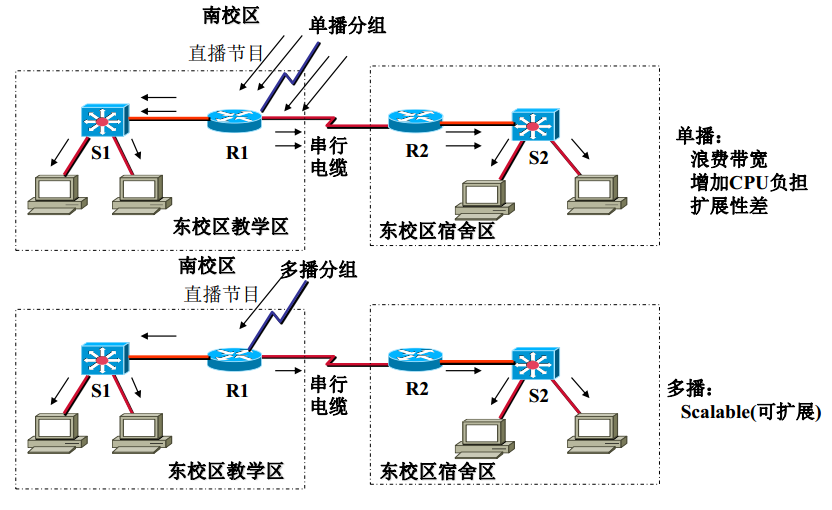
\includegraphics[width=0.8\linewidth]{fig/multicast.png}
\end{figure}

因特网组管理协议(Internet Group Management Protocol, IGMP)用于路由器查询与它直连的网络上是否存在组成员
\begin{itemize}
	\item IGMPv1协议只能对某个接口查询所有组,如果三次查询在十秒内都没有收到响应报告,则认为该接口没有任何组成员。
	\item IGMPv2协议可以直接针对某个组进行查询,而且主机加入组和离开组都要发通告。
\end{itemize}

防止回路
\begin{itemize}
\item 逆向路径广播:指定源的树\\
利用源地址查路由表,如果多播分组从该接口来,则才进行扩散(类DFS)\\
建路由表时源地址路径上一定是最短路径,每一次都往远的地方走,故一定没有回路
\item 逆向路径多播:对于每个多播地址G,每个源地址形成一棵树,即源特定组播树(source-specific multicast tree),然后剪枝\\
如果有新主机加入多播组,则要将路径嫁接回来
\end{itemize}

\begin{itemize}
	\item 稠密(dense):全收,扩散$\to$同样要防回路
	\item 稀疏(sparse)
\end{itemize}

最短路径多点播送生成树(MOSPF):
Steiner树是总代价最小的分布树,但是NP难问题,故采用最短路径

% PIM-Sparse模式
% !TEX root = main.tex

\section{传输层} % transport layer
传输层协议称为\textemph{端到端}或\textemph{进程到进程}的协议。 因特网的传输层可以为两个进程在\textemph{不可靠的网络层}上建立一条\textemph{可靠的逻辑链路},提供\textemph{字节流}传输服务,并且可以进行\textemph{流控制}和\textemph{拥塞控制}。

因特网的传输层有两个协议:
\begin{itemize}
\item UDP协议提供\underline{无连接的不可靠尽力服务}(IP数据报协议字段\textemph{UDP为17})
\item TCP协议提供\underline{面向连接的可靠字节流服务}(IP数据报协议字段\textemph{TCP为6})
\end{itemize}

我们把传输层的数据单元(报文)称为\underline{数据段(segment)}。

每个TCP/UDP连接可以由一个四元组唯一标识:\underline{源IP地址、源端口号、目的IP地址、目的端口号},通过\textemph{端口号}区分不同进程。

而一对\underline{IP地址和端口号}就构成一个通信端点,也被称为\underline{套接字(socket)}。

\begin{itemize}
    \item 知名端口:0-1023,为提供知名网络服务的系统进程所用。如:
    \begin{center}
    \begin{tabular}{|c|c|c|c|}\hline
        80 & HTTP & 25 & SMTP\\\hline
        20 & FTP 数据 & 53 & DNS\\\hline
        21 & FTP 控制 & 110 & POP3\\\hline
        23 & Telnet & &\\\hline
    \end{tabular}
    \end{center}
    \item 注册端口:1024-49151。在IANA注册的专用端口号,为企业软件所用。
    \item 动态端口:49152-65535,没有规定用途的端口号,一般用户可以随意使用。也称为私用或暂用端口号。
\end{itemize}

\subsection{UDP协议}
\subsubsection{概述}
用户数据报协议(User Datagram Protocol, UDP)只提供\textemph{无连接的不可靠的尽力服务}。发送给接收进程的数据有可能\textemph{丢失},也有可能\textemph{错序}。
可以说UDP协议是IP协议的简单扩展,只是在IP协议上增加了\textemph{端口号},把进程关联起来了。
\begin{itemize}
\item UDP是\textemph{面向报文}的传输方式,即应用层交给UDP多长的报文,UDP就照样发送,每一次都发送一个报文。
既不合并,也不拆分,而是\textemph{保留}这些报文的\textemph{边界}。
\item 接收进程每次接收一个完整的数据报,如果进程设置的接收缓冲区不够大,收到的数据报将被截断。
\end{itemize}

\subsubsection{数据段格式}
\begin{figure}[H]
    \centering
    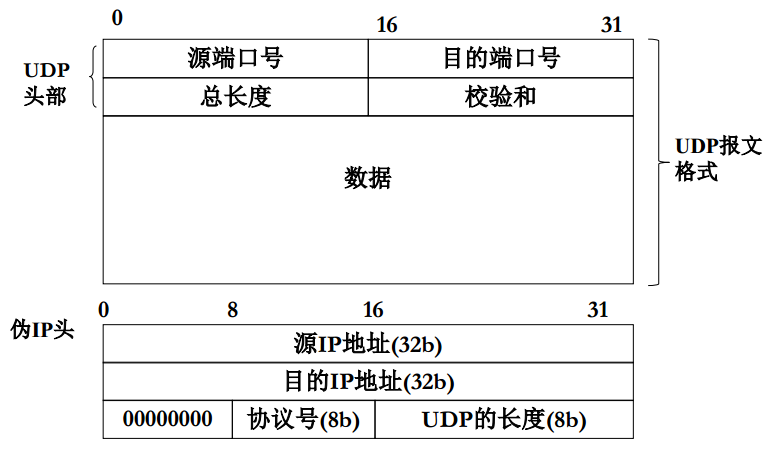
\includegraphics[width=0.6\linewidth]{fig/udp_format.png}
\end{figure}
\begin{itemize}
    \item 总长度:整个UDP报文长度
    \item 源端口号和目的端口号(2B):用于关联发送进程和接收进程
    \item 校验和:由\underline{伪IP头}(只用来算校验和,不进行传递)、\underline{UDP头}(校验和用0填充)和\underline{UDP数据}形成。
    其中,伪IP头的协议号为17。
    如果发送方把校验和设置为0,接收方会忽略校验和。
    UDP长度就是UDP头部填写的总长度。
\end{itemize}

\subsection{TCP协议}
\subsubsection{概述}
传输控制协议(Transmission Control Protocol, TCP)为进程之间提供\textemph{面向连接的可靠的}数据传送服务(通过滑动窗口协议实现)。TCP为\textemph{全双工}协议。TCP提供\textemph{流控制}机制,即控制发送方的发送速度,使发送的数据不会淹没接收方。作为因特网的主要数据发源地,TCP还提供\textemph{拥塞控制}功能。
\begin{figure}[H]
    \centering
    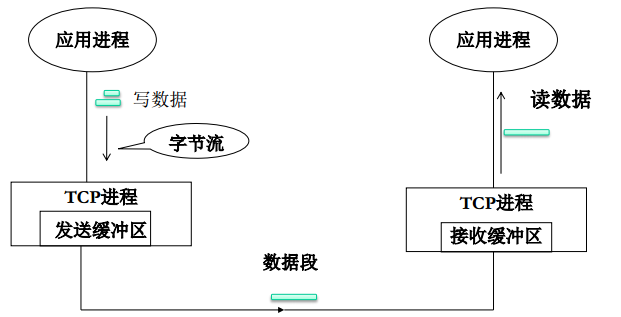
\includegraphics[width=0.5\linewidth]{fig/TCP.PNG}
\end{figure}

\begin{itemize}
\item TCP连接只能在\textemph{两个进程}间建立
\item TCP是\textemph{面向字节流}的传输方式,多次发送的数据可以放在一个数据段中传送且\textemph{不标识边界}。TCP有一个缓冲,当应用程序传送的数据块太长,TCP就可以把它划分短一些再传送。如果应用程序一次只发送一个字节,TCP也可以等待积累有足够多的字节后再构成报文段发送出去。(注意上图,是将两条写数据合并在一起变为一个数据段才发送)
\item TCP连接提供\textemph{可靠的无比特错的数据传送},但经过因特网可能出现\textemph{丢失和错序(同UDP)}。
\item 每个\textemph{数据段数据部分}的\textemph{最大长度(字节)}不能超过MSS(Maximum Segment Size)\footnote{一般来讲,TCP协议会以最大传输单元(MTU,帧的数据部分)减去IP头和TCP头作为MSS。如果是以太网,则是$1500-20-20=1460$。}。
\item 客户端通过查路由表知道\textemph{IP地址},\textemph{端口号}自动选一个未用的
\end{itemize}

\subsubsection{数据段格式}
\begin{figure}[H]
    \centering
    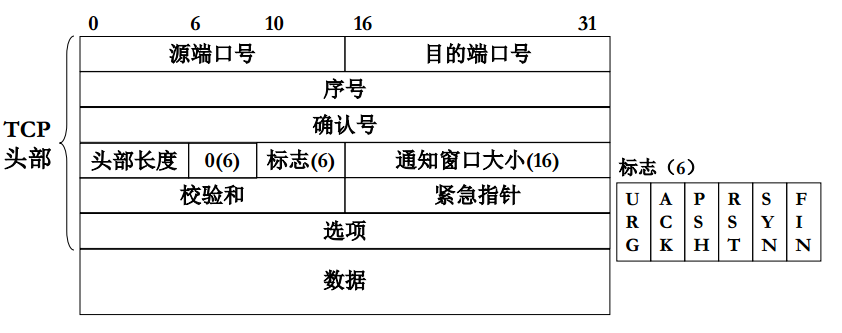
\includegraphics[width=0.8\linewidth]{fig/tcp_format.png}
\end{figure}
\begin{itemize}
    \item 序号:字节流中的\textemph{每个字节}都会被编号。
    \underline{初始序号}(initial sequence number, ISN)采用基于时间的方案, 一般采用\textemph{随机数}。
    数据部分的第一个字节的编号为\textemph{ISN+1}。
    \item 头部长度:以\textemph{字(32b)}为单位,同IP数据报。
    \item 标志:标记为1时有效
\begin{itemize}
\item SYN:同步序号标志,用来发起一个TCP连接
\item FIN:表示关闭连接,\textemph{不再发送数据},但是可以接收数据,也可以发送\textemph{数据段}(不包含数据)
\item ACK:表示确认号有效
\item PSH:告知接收方发送方执行了推送(Push)操作,接收方需要尽快将所有缓存的数据交给接收进程
\item RST:发现连接可能出了问题,连接重置
\item URG:紧急指针标志位
\end{itemize}
    \item 通知窗口(advertised window, advWin)大小:接收方告知发送方,发送方据此做出调整
    \item 校验和:由\underline{伪IP头、TCP头和TCP数据部分}形成,其形成方法与UDP协议类似。伪IP头的协议字段值为6。
    \item 紧急指针:用于指出紧急/\underline{带外数据}(out-of-band, OOB)\footnote{带外数据不属于字节流}的边界,即紧急数据的\textemph{最后一个字节的偏移量}。标志URG为1时有效。
    \begin{figure}[H]
        \centering
        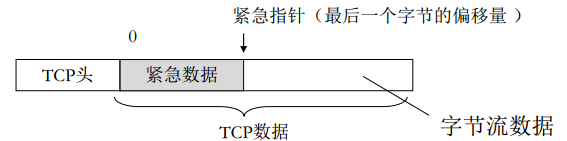
\includegraphics[width=0.5\linewidth]{fig/out-of-band.png}
    \end{figure}
    \item 选项:建立连接时有MSS、窗口比例(Scale)、是否使用选择性确认(SACK-Permitted)等。数据传送时有选择性确认的序号范围(Seletive ACK, SACK)、时间戳等。
\end{itemize}

\subsubsection{工作过程}
\begin{center}
    \begin{tikzcd}
        \text{建立连接}\arrow{r} & \text{传送数据}\arrow{r} & \text{释放连接}
    \end{tikzcd}
\end{center}
\begin{itemize}
    \item 建立连接:\textemph{非对称}活动,服务器一直在等,客户向服务器呼叫
    \item 传送数据:\textemph{全双工}方式
    \item 释放连接:\textemph{对称}活动,可由任何一方发起
\end{itemize}

\myhline
\begin{figure}[H]
    \centering
    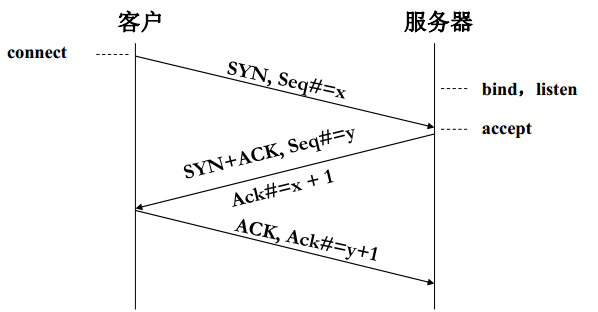
\includegraphics[width=0.6\linewidth]{fig/tcp_connect.png}
    \caption*{\textbf{三次握手建立连接}}
\end{figure}
\begin{itemize}
    \item 客户端需要知道服务器的IP地址和端口号。
    服务器收到客户端发来的连接请求(SYN报文)后
    \begin{enumerate}
        \item 查看是否有进程监听该端口。
        若有,则将此连接请求传给该进程;否则,服务器发RST拒绝它。
        \item 如果该进程接受连接请求,则发回SYN+ACK报文。
    \end{enumerate}
    \item 每一步均采用\textemph{超时重传},多次重发后将放弃。重发次数与间隔时间依系统不同而不同。
    \item x和y为初始序号(随机数),分别用于两个方向的数据传送。两个方向的下一个数据段的序号分别为x+1和y+1。
    \item 注意这里确认号含义与数据链路层不同,传输层的确认号是\textcolor{red}{\textemph{期待接收下一个字节}}的序号
\end{itemize}

\begin{example}
    为什么需要三次握手建立连接?
\end{example}
\begin{analysis}
    只有一次握手的话,也就是说客户端只要发送了连接请求就认为TCP已连接,也许服务器根本就不存在或者没打开。如果继续发送数据的话,浪费带宽。再说客户端也需要服务器传来的初始序号和很多选项,这个都做不到。

    如果采用两次握手,则客户端可以通过发送大量伪造的源地址连接请求,经过两次握手后服务器误以为连接已经建立,最终耗尽所有资源,使得合法的请求连接都被拒绝,无法提供正常的服务,此即DoS攻击的原理。

    即使是三次握手也无法避免DoS攻击和DDoS攻击,因为依然可以实现大量客户端同时向服务器发送连接请求,然后接收下服务器发来的确认数据包后,不再向服务器发送确认数据包(即客户端主动不进行第三次握手),那么服务器在短时间内会维护这样的半连接队列,等待队列中的客户端确认。但由于每个半连接都会耗费服务器的资源,故最终会导致资源不够用,拒绝正常的连接请求,使得正常服务无法提供。

    预防DDoS的方法:限制同时打开SYN半连接的数目,缩短SYN半连接超时时间,关闭不必要的服务。
\end{analysis}

\myhline
TCP协议传输数据采用\textemph{选择性确认}协议(\textemph{滑动窗口}),不使用NAK。只有\textemph{一个超时定时器}。
采用字节流方式,每个数据段使用其\textemph{第一个字节}的编号作为序号,按\textemph{字节}编号。

注意TCP协议中没有说明如何处理错序到达的数据段,要取决于具体实现。

\begin{figure}[H]
    \centering
    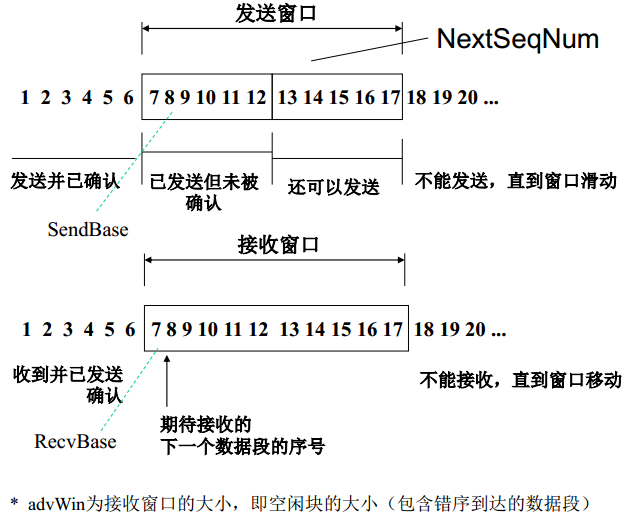
\includegraphics[width=0.6\linewidth]{fig/TCP-window.PNG}
\end{figure}
\begin{itemize}
\item 接收方先传MSS,x和接收/通知窗口大小(advWin)
\item 发送方做发送窗口,序号为x+1,大小等同advWin(接收窗口和发送窗口大小\textemph{都会改变},流控制)
\item 若接收缓冲区已满,则要等接收方进程将缓冲区取空,发送方才能继续发,否则发送窗口大小始终为0
\item 超时定时器会自动移动
\end{itemize}

\begin{example}
    下图为一个普通TCP连接的数据传送图(不使用Nagle Algorithm,Delayed ACK,Fast Retransmission,Slow start等),请填空
    \begin{figure}[H]
        \centering
        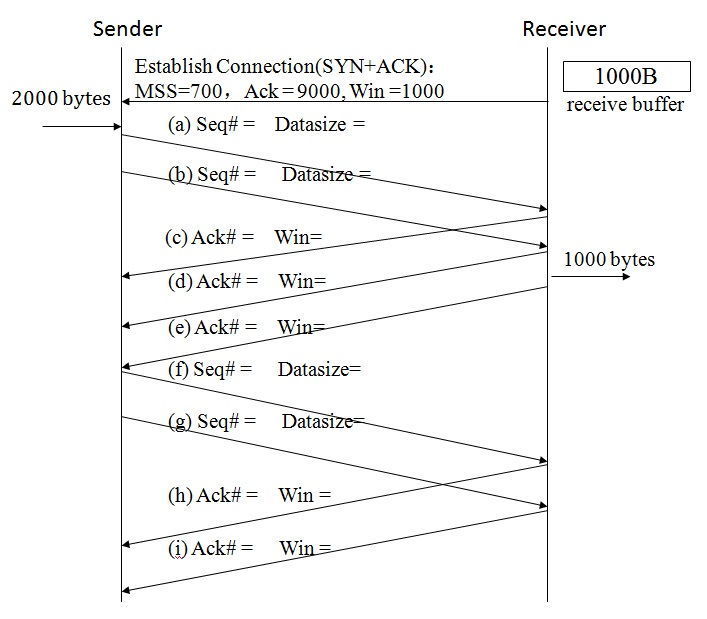
\includegraphics[width=0.5\linewidth]{fig/tcp_example.jpg}
    \end{figure}
\end{example}
\begin{analysis}
    注意每次发送数据最多就只有MSS,但发送窗口大小可以大于MSS。
    \begin{enumerate}[label=(\alph*)]
        \item 9000 700,取初始序号作为Seq初值,\underline{advWin}作为\underline{sendWin初值}。发送数据段大小为\underline{MSS},因为MSS小于滑动窗口大小。
        \item 9700 300,继续将发送窗口内的字节发光,此时sendWin还是1000,只是里面的字节都已发送但未确认而已
        \item 9700 300,期待接收序号为9700,advWin减为$1000-700=300$
        \item 10000 0,期待收10000,advWin减为0,进而sendWin减为0
        \item 10000 1000,取走1000,故advWin恢复,发ACK
        \item 10000 700,重复(a)(b)(c)(d)过程
        \item 10700 300
        \item 10700 300
        \item 11000 0
    \end{enumerate}
\end{analysis}

\myhline
\begin{figure}[H]
    \centering
    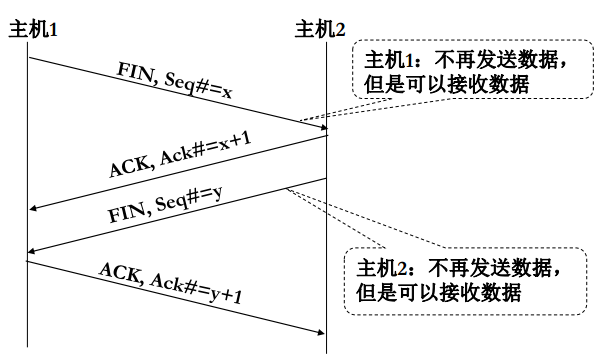
\includegraphics[width=0.6\linewidth]{fig/tcp_close.png}
    \caption*{\textbf{四次握手关闭连接}}
\end{figure}
\begin{itemize}
    \item FIN报文采用\textemph{超时自动重发}方式。在若干次重发后依然没有收到确认,则发送RST报文给对方后强行关闭连接。不同的系统重发方法不同。x和y都是\textemph{上一个收到的数据段的确认号}。
    \item 先发送FIN报文的一方在ACK发送完毕后需要等待\textemph{2MSL}(Maximum Segment Lifetime)的时间才\textemph{完全关闭}连接(占用端口号),用于\textemph{等待该连接的数据在因特网中消失}。TCP标准中MSL采用60秒,Unix采用30秒。
    \item 可以合并中间两次握手(ACK和FIN)或两方同时发出ACK。
\end{itemize}

\myhline
\begin{figure}[H]
    \centering
    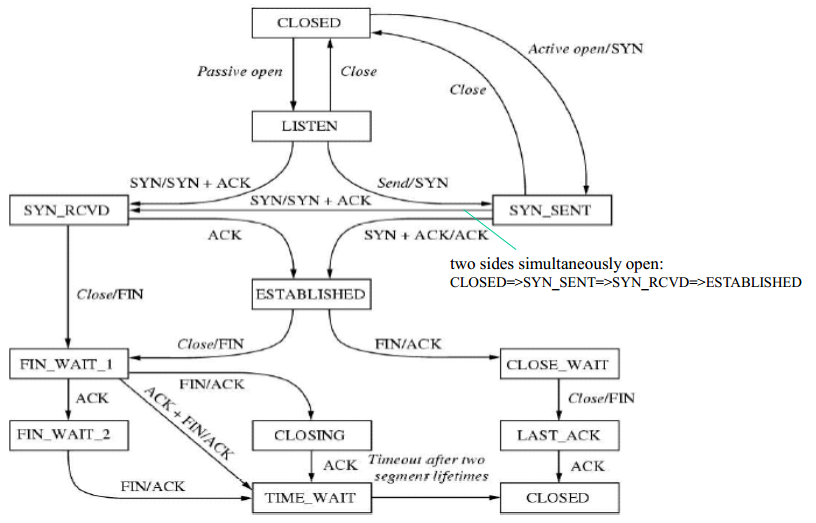
\includegraphics[width=0.8\linewidth]{fig/TCP-transition.PNG}
    \caption*{TCP协议状态转移图}
\end{figure}

\subsubsection{重传机制}
数据链路层每个帧都有一个超时定时器,而传输层只有\textemph{一个超时定时器}。
\begin{itemize}
\item \underline{快速重传}(fast retransmit):如果发送方收到一个数据段的\textemph{3次重复的ACK}(包括第一次则一共4次),它就认为其后的数据段(由确认号指出)已经丢失,在超时之前会重传该数据段。
缺点是丢包时间很长,优点是可以减缓网络压力。
\item \underline{延迟确认}(delayed ACK):接收方并不在收到数据段立即进行确认,而是延迟一段时间再确认。如果这个期间收到多个数据段,则只需要发送一个确认。
如果在这个期间接收方有数据帧要发往发送方,还可以使用捎带确认(piggybacking)。
大部分的系统(Windows/Unix)的延迟确认时间为200毫秒。TCP标准要求延迟确认不大于500毫秒。
\item \underline{选择性确认}:接收方把收到的数据块通过数据段的选项告知发送方,使发送方不会重传这些数据块
\begin{figure}[H]
    \centering
    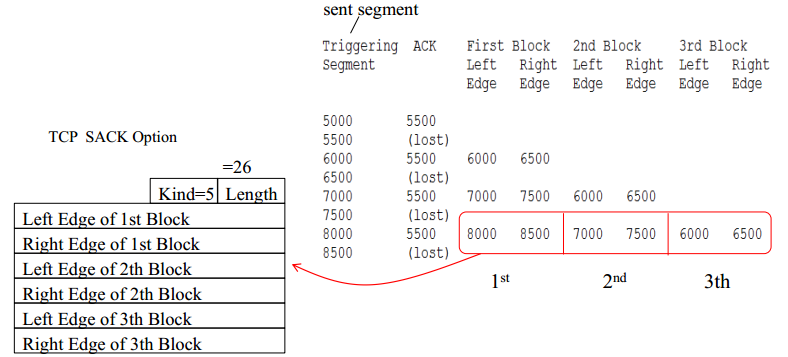
\includegraphics[width=0.8\linewidth]{fig/SACK.PNG}
\end{figure}
\end{itemize}

\subsubsection{传输层与数据链路层比较}
\begin{center}
    传输层滑动窗口协议和数据链路层的区别
\begin{tabular}{|c|c|c|}\hline
     & 传输层 & 数据链路层\\\hline
    序号 & 随机初始序号+1,按字节计数 & 每一个帧一个序号 \\\hline
确认号 & 期待接收的序号 & \begin{tabular}{l}收到哪一个就确认哪一个\\代表当前与之前的全收到了\end{tabular}\\\hline
窗口大小 & 会改变 & 不会改变\\\hline
超时定时器 & \begin{tabular}{l}只有一个,只要有未确认的数据段\\就会启动(针对未确认序号最小的);\\超时没收到确认,就会重传\end{tabular} & 每个帧都有一个\\\hline
\end{tabular}
\end{center}

\subsubsection{超时计算}
数据链路层的回退N协议由于没有中间节点,故可以用固定的超时时间(1RTT)。
而传输层涉及多个节点,故需要实时变化,进行估计。

\textbf{原始公式/指数加权移动平均方法}(Exponentially Weighted Moving Average, EWMA)
\[\begin{aligned}
    \text{EstimatedRTT} &= (1-\alpha)\times \text{EstimatedRTT} + \alpha \times \text{SampleRTT}\\
    \text{RTO} &= 2\times \text{EstimatedRTT}
\end{aligned}\]
RTO(retransmission timeout)为超时时间,$0<\alpha<1$,$\alpha$越小过去样本的影响越大。
一般取值$\alpha=0.9$,这会使过去影响指数减少。

\myhline
TCP超时计算最常用的算法---\textbf{Jacobson算法}
\[\begin{aligned}
    \text{EstimatedRTT} &= (1-\alpha)\times \text{EstimatedRTT} + \alpha \times \text{SampleRTT}\\
    \text{DevRTT} &=(1-\beta)\times\text{DevRTT} + \beta\times|\text{SampleRTT}-\text{EstimatedRTT}|\\
    \text{RTO} &= \text{EstimatedRTT} + 4\times \text{DevRTT}
\end{aligned}\]
在RTO计算加上一个合适的安全边际(safety margin),使得在样本变化较大时RTO会很快变得更大(先估计偏移RTT)。
取$\alpha=1/8$,$\beta = 1/4$。
如果发送窗口为12MSS,则每12个段取样一次(采样频率)。

\myhline
\textbf{Karn算法}:在收到重传段确认时不要计算EstimatedRTT,直接计算RTO。
\[\text{RTO} = \gamma\times\text{RTO}\]
而是在每次重传时\textemph{直接把RTO加倍}($\gamma=2$)\textemph{直到数据段首次得到确认},并把这个RTO作为后续段的RTO。
在12次重传后TCP协议发送RST并关闭连接。

\begin{example}
    如果只有最后三个连续发送的数据段被丢失,其它数据段全部收到且RTT一直保持20ms, 从这三个数据段的第一个数据段发送开始计时,还需要多少时间(ms)才可以全部收到这三个数据段的确认?
\end{example}
\begin{analysis}
    一个TCP连接的发送方只有一个超时定时器,只针对未收到确认的第一个数据段启动。\\
    采用Karn算法,第一个数据段RTO 20 + 重传时间RTT 20 = 40ms\\
    收到重传数据段确认,超时定时器移动,同时RTO加倍为40 + 重传时间RTT 20 = 60ms\\
    收到重传数据段确认,超时定时器移动,RTO加倍为80 + 重传时间RTT 20 = 100ms\\
    总数为$40+60+100=200$ms
\end{analysis}

\subsubsection{拥塞控制}
\begin{itemize}
\item 流控制:单一发送方和接收方,控制发送的速度,防止太多数据涌向\textemph{接收方}
\item 拥塞控制:防止太多数据涌向\textemph{网络},表现为\underline{丢包}(路由器上缓冲区溢出)和\underline{长延迟}(在路由器缓冲区中排队)
\end{itemize}

\myhline
拥塞控制的两大类方法:
\begin{enumerate}
    \item 端到端的拥塞控制:
\begin{itemize}
    \item 没有来自网络的明确的反馈
    \item 终端系统通过丢包和延迟推导的拥塞
    \item TCP协议的方法
\end{itemize}
    \item 网络辅助的拥塞控制:
\begin{itemize}
    \item 路由器反馈给终端系统
    \item 用一个比特指出拥塞发生(SNA, DECbit, TCP/IP ECN, ATM)
    \item 向发送方给一个明确的发送速率
\end{itemize}
\end{enumerate}
* 不主张发送ICMP包,会加重拥塞;应靠TCP自己发现拥塞。

TCP的拥塞控制属于\textemph{端到端的拥塞控制}
\begin{itemize}
    \item \underline{超时}或\underline{收到3个重复ACK}就认为丢包了(同快速重传),看作拥塞发生
    \item TCP协议通过降低发送速率来控制拥塞。发送速率与发送窗口大小有关:
\[\text{发送速率(rate) $=$ SWS(Sending Window Size) $/$ RTT}\]
    \item 通过引入\textemph{拥塞窗口变量CongWin}来限制SWS。
\[\text{SWS} = \min\{\text{CongWin}, \text{AdvWin}\}\]
    CongWin为发送窗口的流量控制,AdvWin为接收方要求的流量控制
\end{itemize}

\myhline
TCP协议改变CongWin的几种机制:
\begin{itemize}
    \item 加性增乘性减(AIMD):发生拥塞\textemph{立即减半},然后\textemph{线性增长}
    \begin{figure}[H]
        \centering
        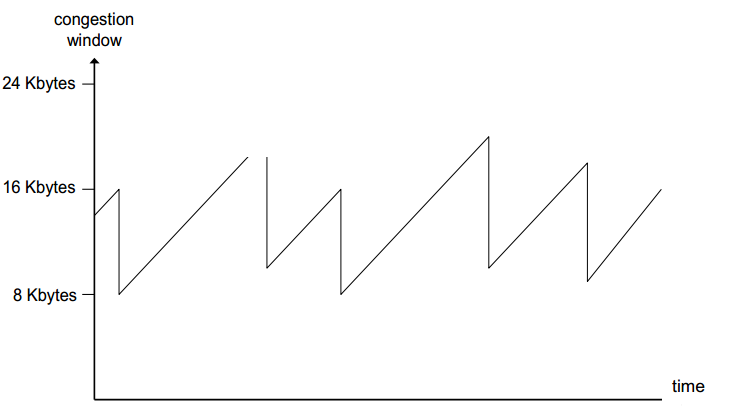
\includegraphics[width=0.5\linewidth]{fig/congression-AIMD.PNG}
    \end{figure}
    \item \underline{慢启动(slow start):Tahoe算法}
    \begin{figure}[H]
        \centering
        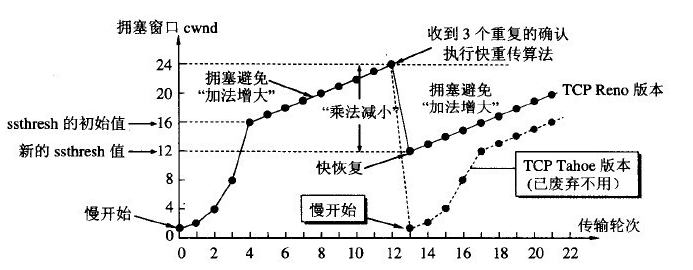
\includegraphics[width=0.8\linewidth]{fig/congression-slow-start.PNG}
    \end{figure}
    假设算法开始时通知窗口大小AdvWin=65535(用系统参数\verb'TCP_MaxWin'(一般为65535)限制CongWin的大小),SegSize为被确认的数据段的大小。
    超时或收到3个重复ACK就会触发快速重传及CongWin的变化
    \begin{enumerate}
        \item 初始时,CongWin设为1MSS, 阈值(threshold)设为65535, 发送一个数据段。
        \item 在当前窗口所有数据段的确认都收到之后, CongWin加倍。
        实际上,每收到一个确认,CongWin增加一个MSS。把它称为慢启动(slow start)是因为这个方法比立即采用advWin更慢。
        \item 当拥塞发生时,把\textemph{当前CongWin(或SWS)的一半}保存为阈值,然后CongWin又从1MSS开始慢启动(时刻0就是1MSS,上图有误)。
        \item 当CongWin增长到等于或大于阈值时,在当前窗口所有数据段的确认都收到之后, CongWin增加一个MSS(拥塞避免)。
        实际上,每收到一个ACK,CongWin增加$\text{SegSize} / \text{CongWin}$。
        如果发生拥塞,转(3)。
    \end{enumerate}
    \item \underline{快速恢复(fast recovery):Reno算法}\\
    从原来CongWin的一半开始线性增长(时刻0就是一半CongWin)
\end{itemize}

\subsubsection{存在的问题}
\textbf{问题零---关闭连接后立即又生成新的连接导致错乱}

\bigskip
\textemph{随机初始序号}和\textemph{2MSL}都用于阻止重建TCP连接相同4元组,不会收到上一次连接遗留的数据的干扰

\myhline
\textbf{问题一---长肥管道}:带宽大
\[\text{未确认的数据量capacity(b)} = \text{bandwidth(b/s)} \times \text{RTT(s)}\]
\begin{itemize}
\item \textemph{序号回绕}问题(因为速度太快):使用一般数据段的选项\verb'timestamp'(TS)。只用于区分回绕的序号是不同的,不用于确定先后次序。
也可以用Window scaling的方法,在SYN数据段选项设置WinScale(取值0-14, 默认值为0)
\[\text{sendWin} = \text{advWin} * 2^{\text{WinScale}}\]
\item \textemph{发送窗口太小},满足不了需求:当丢包发生时,由于SWS的限制,管道将会被清空。解决方法:快速重传、快速恢复。(数据链路不会,因为直连网)
\end{itemize}

\myhline
\textbf{问题二---死锁现象}:sendWin为0,接收方取空,再发不为空的ACK丢失了。
缓冲区不变化,不会发确认回来。
解决方案:
\begin{itemize}
\item 接收方可以启动一个超时定时器,可以是可以,但如果发送方没有数据传了,那接收方还是会继续发。(无谓发送数据)
\item 一般从发送方解决:在发送窗口为0之后,并且发送方有数据要发送,则启动坚持定时器(Persist Timer),定期从要发送的数据中取一个字节发送出去(Window Probe),直到收到不为0的通知窗口为止
\end{itemize}

\myhline
\textbf{问题三---傻瓜窗口症候}(silly window syndrome)
\begin{itemize}
    \item 发送进程有很多小批量数据要发送,如用telnet作为远程终端\\
    \underline{Nagle算法}---启发式算法(类似于停等协议)
    \begin{figure}[H]
        \centering
        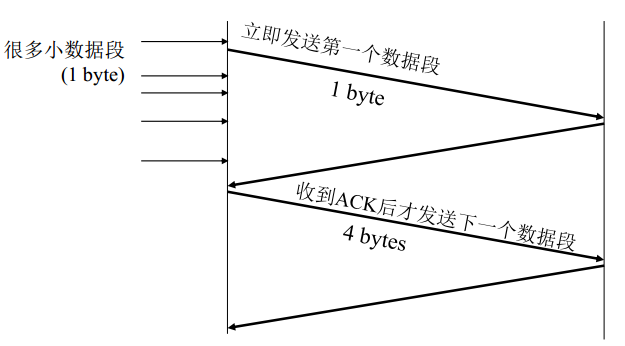
\includegraphics[width=0.6\linewidth]{fig/nagle.PNG}
    \end{figure}
    \begin{enumerate}
        \item 立即发送一个数据段,即使发送缓冲区只有一个字节
        \item 只有收到\underline{上一个数据段的确认}(此时缓冲区已经积累一定数据)或者\\\underline{发送缓冲区中数据超过MSS},才可以发送下一个数据段
        \item 对于即时性要求高的地方,如Window方式的鼠标操作,要\textemph{关闭}Nagle算法
    \end{enumerate}
    \item 接收进程频繁取走小批量数据\\
    \underline{Clark算法}:要等到接收缓冲区的空闲块大小为\underline{接收缓冲区大小的一半}\\或\underline{达到MSS}时才发送确认。
\end{itemize}

\subsubsection{定时器}
\begin{itemize}
\item 每个连接只针对第一个未确认数据段启动\underline{重传定时器}(retransmission timer)。所有数据段都已确认,则关闭它。超时重传或发送窗口移动时要重启该定时器。
\item \underline{坚持定时器}(persist timer)用于保持信息流动,即使另一端关闭了接收窗口。
\item \underline{保活定时器}(keep-alive timer)在\textemph{长时间}没有交换数据段之后,用于检测连接的另一端是否出了问题。(如微信)隔2个小时,发10个数据段,如果没有ACK则关闭连接。(由应用层程序来做而不是TCP)
\end{itemize}

\subsection{TCP与UDP比较}
\begin{center}
\begin{tabular}{|c|c|c|}\hline
 & TCP & UDP\\\hline
连接 & 面向连接 & 无连接\\\hline
传输可靠性 & 可靠的 & 不可靠的\\\hline
消息 & 面向字节流 & 面向报文\\\hline
通信模式 & 只支持点对点 & 支持一对一、多对多、多对一、多对多\\\hline
拥塞控制 & 有 & 无\\\hline
系统资源/开销 & 大 & 小\\\hline
\end{tabular}
\end{center}

当数据传输的性能必须让位于数据传输的\textemph{完整性}、可控制性和可靠性时,TCP是更好的选择;
反之,当强调\textemph{传输性能}而不是传输的完整性时,如:音频和多媒体应用,UDP是最好的选择。
% !TEX root = main.tex

\section{应用层}
应用层协议一般都是采用客户-服务器结构
\begin{center}
\begin{tabular}{|c|c|c|c|}\hline
应用 & 应用层协议 & 传输层协议 & 端口号\\\hline
Email & SMTP [RFC 2821] & TCP & 25\\\hline
远程终端访问 & Telnet [RFC 854] & TCP & -\\\hline
Web & HTTP [RFC 2616] & TCP & -\\\hline
文件传输 & FTP [RFC 959] & TCP & 21\\\hline
域名解析服务 & DNS & UDP & 53\\\hline
简单网络管理协议 & SNMP & UDP & 161\\\hline
\end{tabular}
\end{center}

\subsection{HTTP协议}
\subsubsection{概述}
\begin{itemize}
\item 网页(Web page)是由对象(objects)构成的。这些对象可以是HTML文件、 JPEG图像文件、 MP4视频文件等。
\item 网页的HTML文件中指出了所需的其他对象。
\item 每个对象采用URL指明存放地址。URL由\underline{主机名}和\underline{路径名}构成。
\end{itemize}

HTTP: 超文本传送协议(hypertext transfer protocol),是无状态的(stateless),server不保留过往客户端的任何信息
\begin{itemize}
\item 非持续连接的HTTP:每个时刻最多请求一个Web对象,每建立一个连接最多只能传送一个Web对象。\verb'connection: close'
\item 非流水式持续连接HTTP:每个时刻可以请求多个Web对象,每建立一个连接可以传送多个Web对象。\verb'connection: keep-alive'
\begin{figure}[H]
    \centering
    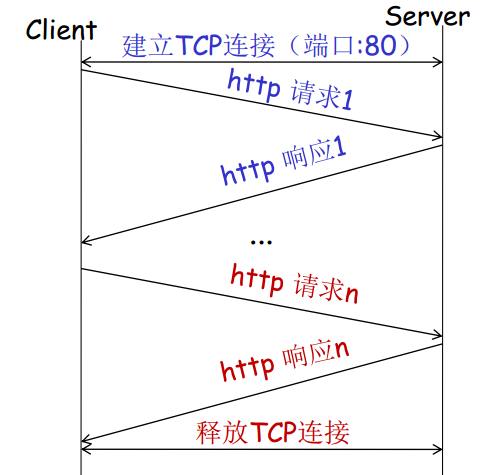
\includegraphics[width=0.4\linewidth]{fig/non-pipelining-http.png}
\end{figure}
\item 流水式持久连接HTTP:可以连续请求多个Web对象,每建立一个TCP连接可以传送多个Web对象。HTTP/1.1 默认使用持续连接。\verb'connection: keep-alive'
\begin{figure}[H]
    \centering
    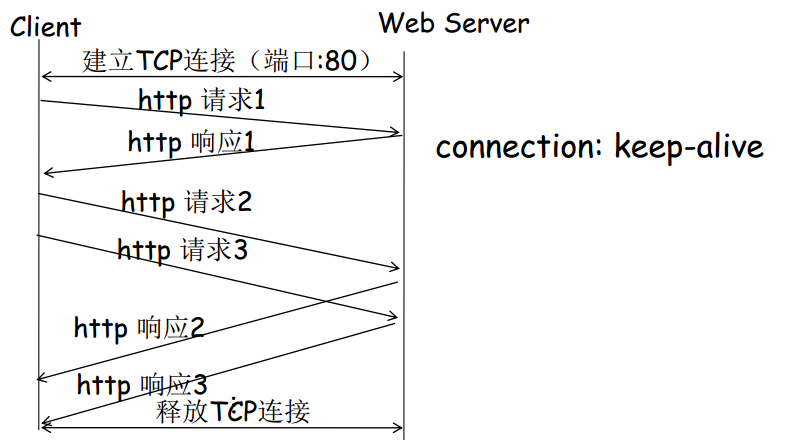
\includegraphics[width=0.6\linewidth]{fig/pipelining-http.png}
\end{figure}
\end{itemize}

\subsubsection{消息}
HTTP请求消息(message)
\begin{figure}[H]
    \centering
    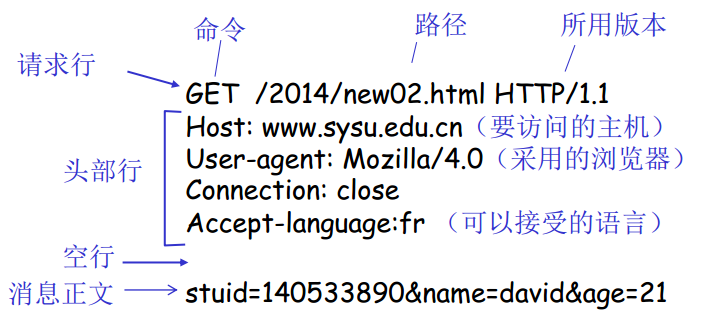
\includegraphics[width=0.6\linewidth]{fig/http-msg.png}
\end{figure}
\begin{itemize}
\item 只有POST命令才有消息正文
\item 每一行均以回车换行结束(\verb'\r\n'),这一点很重要,否则收不到回复!
\end{itemize}

HTTP响应信息
\begin{figure}[H]
    \centering
    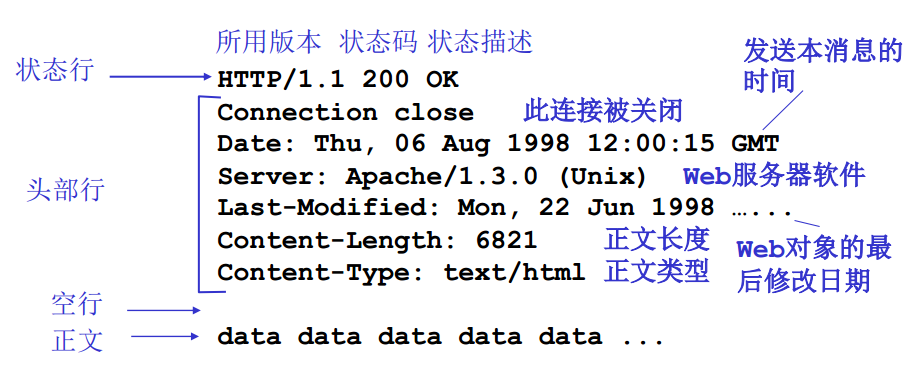
\includegraphics[width=0.6\linewidth]{fig/http-respond.png}
\end{figure}

用telnet建立TCP连接,然后发送GET请求,如
\begin{lstlisting}
telnet www.sysu.edu.cn 80
GET /2012/cn/index.htm HTTP/1.1
Connection: close
Host: www.sysu.edu.cn
\end{lstlisting}

\subsubsection{HTTP版本更新}
HTTP1.1对HTTP1.0的改进:
\begin{enumerate}
\item 一个TCP连接可以传送多个HTTP请求和响应。
\item 可以采用流水线方式,即多个请求和响应过程可以重叠。
\item 增加了更多的请求头和响应头。
\end{enumerate}

HTTP2.0
\begin{enumerate}
\item 采用二进制格式,而非文本格式
\item 完全多路复用,而非有序并阻塞的
\item 使用报头压缩来降低开销
\item 让服务器可以将响应主动推送到客户端缓存中
\end{enumerate}

\subsection{FTP协议}
\begin{figure}[H]
\centering
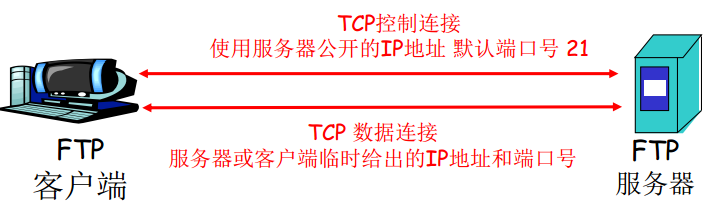
\includegraphics[width=0.6\linewidth]{fig/FTP.png}
\end{figure}

\begin{itemize}
\item 使用FTP协议首先建立\textemph{控制连接},然后建立\textemph{数据连接},客户端再通过控制连接发出命令,通过数据连接得到服务器返回的结果或上传数据给服务器。
\item 控制连接为带外数据(\verb'out of band')
\item FTP服务器会保留状态: 当前目录、已做的认证
\end{itemize}

如下例,得到IP地址(\verb'202.116.86.101')后,计算端口号(12*256+26=3098),\\
进而建立数据连接\verb'telnet 202.116.86.101 3098'
\begin{lstlisting}
telnet 202.116.86.101 21
220 Microsoft FTP Service
user net
331 Password required for user.
pass 123456
230 User user logged in.
pasv
227 Entering Passive Mode (202,116,86,101,12,26).
list
125 Data connection already open; Transfer starting.
226 Transfer complete.
quit
221
\end{lstlisting}

\subsection{Email协议}
Email有三个主要组件:
\begin{itemize}
\item 用户代理(user agents)
\item 邮件服务器(mail servers)
\item 简单邮件传送协议(simple mail transfer protocol, SMTP):TCP端口号25
\end{itemize}
\begin{figure}[H]
\centering
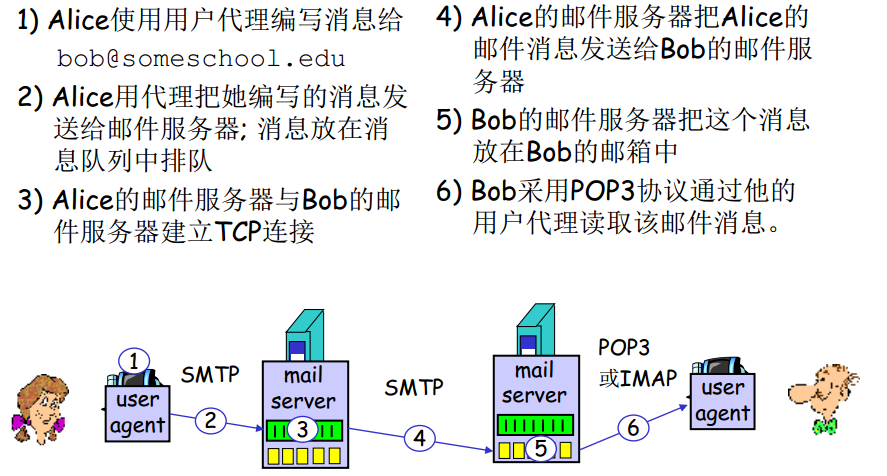
\includegraphics[width=0.7\linewidth]{fig/SMTP.png}
\end{figure}

\subsection{域名系统}
\subsubsection{概述}
域名系统(Domain Name System, DNS)提供的服务
\begin{itemize}
\item 主机名到IP地址的转换
\item 为主机取别名
\item 权威名(Canonical name)、别名(alias names)
\item 为邮件服务器取别名
\item  负载分配(load distribution)
\item 重复的Web服务器: 一个权威名对应一组IP地址
\end{itemize}

\myhline
不采用集中式DNS的原因:不易扩大规模
\begin{itemize}
\item 单点失效
\item 流量过于集中
\item 可能距离数据库太远
\item 维护问题
\end{itemize}

\subsubsection{DNS服务器}
根名字服务器
\begin{itemize}
\item 公开的IP地址,不需要解析名字,由本地名字服务器直接联系
\item 根名字服务器:如果不知道名字映射,把该名字所在的权威名字服务器的IP地址返回给本地名字服务器
\item 根服务器主要用来管理互联网的主目录,全世界只有13台:1个为主根服务器,放置在美国。其余12个均为辅根服务器,其中9个放置在美国,欧洲2个,位于英国和瑞典,亚洲1个,位于日本。
\end{itemize}

权威服务器
\begin{itemize}
\item 顶级域名提供了权威DNS服务器的IP地址,包括com, org, net, edu, uk, fr, ca, jp等
\item 权威DNS服务器:
\begin{itemize}
\item 每个组织机构的公开可访问主机都必须提供公共可访问的DNS记录,这些记录保存在权威DNS服务器上,并把这些主机的主机名映射到IP地址上(e.g., Web, mail).
\item 权威服务器由大型组织或服务提供商维护
\end{itemize}
\end{itemize}

\begin{figure}[H]
    \centering
    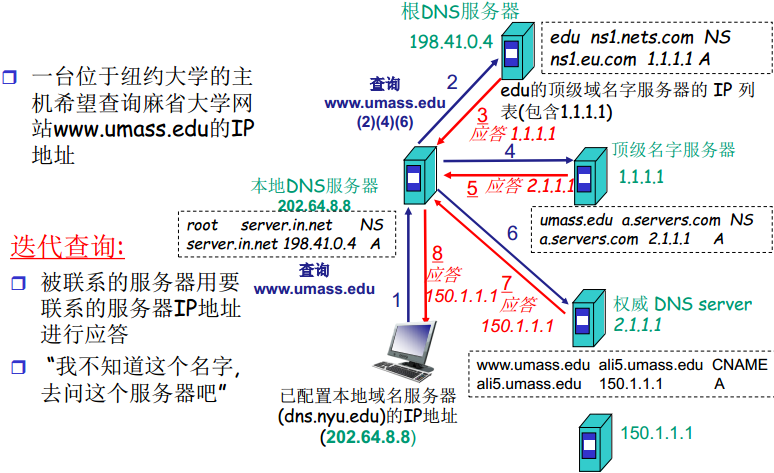
\includegraphics[width=0.8\linewidth]{fig/dns-example.png}
\end{figure}

\subsubsection{资源记录}
采用分布数据库保存资源记录(resource records, RR)
\[\text{(name, value, type, class,ttl)}\]
\begin{itemize}
\item Type=A (Address RR)
\begin{itemize}
\item name是主机名
\item value是IPv4地址
\end{itemize}
\item Type=CNAME
\begin{itemize}
\item name是别名
\item 值是规范名(canonical name)或真名(the real name):
例如, www.jazz.com是主机bp2.jazz.com的别名
\end{itemize}
\end{itemize}

\section{其他内容}
\subsection{无线局域网}
\subsubsection{基本特性}
无线局域网(WiFi)IEEE 802.11
\begin{itemize}
\item 不同标准MAC层一样,改进的是\textemph{物理层}(发、编码、怎么收)
\item 无线信道特点:信号衰减快、抗干扰能力差、发送速率慢、共享信道有限带宽
\end{itemize}
\begin{figure}[H]
    \centering
    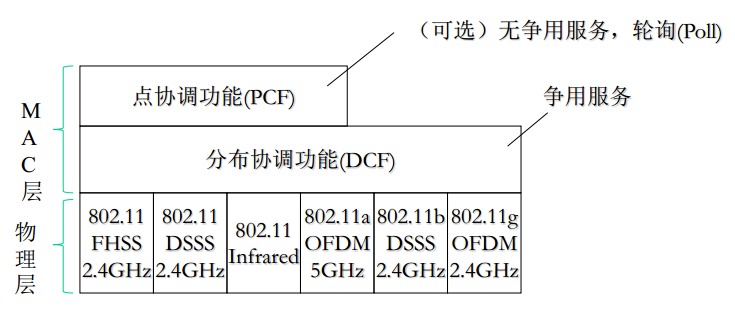
\includegraphics[width=0.6\linewidth]{fig/802-11.png}
\end{figure}

MAC层一般用分布协调功能(DCF)
\begin{itemize}
\item 原子操作:发完数据等待28$\mu$s后才发ACK
\item CSMA/CA(Carrier Avoidance)算法:尽可能少冲突,尽可能少重传;即使空闲也要随机等一段时间
\end{itemize}

\subsubsection{设施}
\begin{itemize}
\item 无固定设施(自组织IBSS):独立基本服务集(Basic Service Set, BSS),不需要路由器,可以几台PC直接连
\item 有固定设施:有个接入点(Access Point, AP),有路由器,连成基本服务集;
扩展的服务集(ESS),完全无缝连接,自动迁移到下一个AP
\end{itemize}

\subsubsection{帧格式}
\begin{figure}[H]
    \centering
    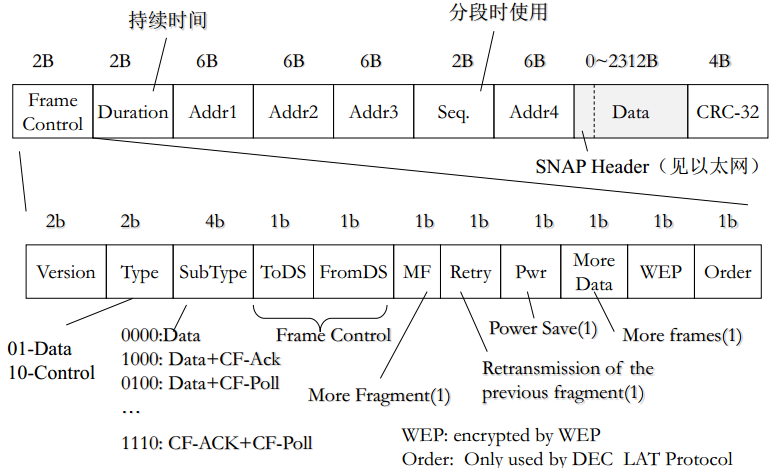
\includegraphics[width=0.8\linewidth]{fig/802-11-frame.png}
\end{figure}

802.11的帧一共有\textemph{4个地址},并没有指出上层协议的部分,所以数据部分(payload)加了\textemph{SNAP}的头部,里面包含了类型指明上层协议。

\begin{figure}[H]
    \centering
    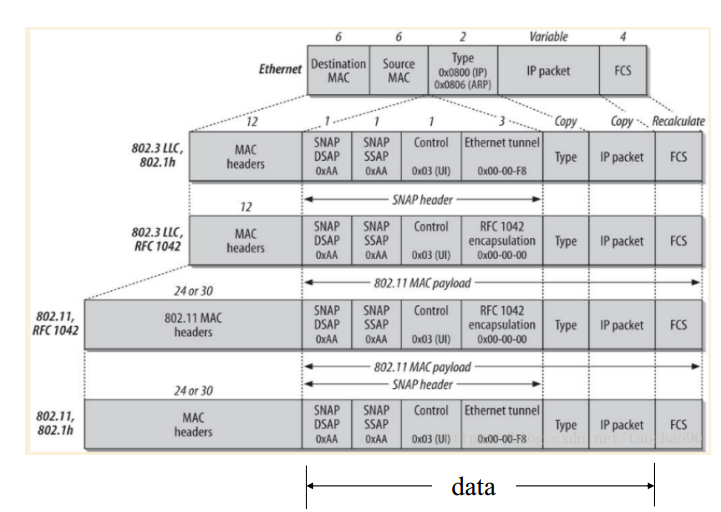
\includegraphics[width=0.8\linewidth]{fig/802-11-frame-2.png}
\end{figure}
\begin{figure}[H]
    \centering
    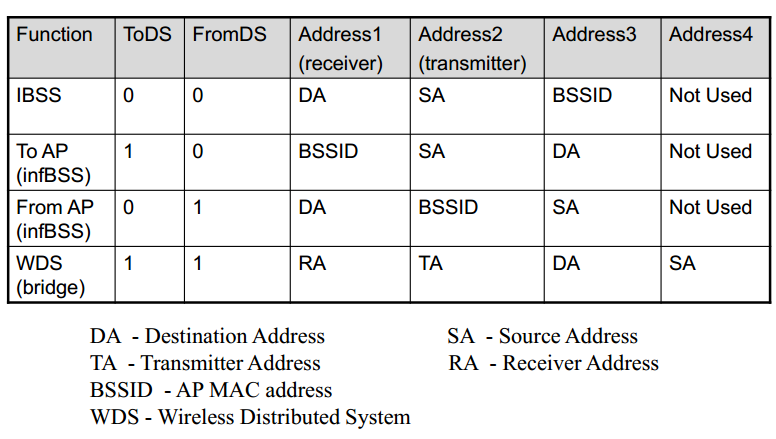
\includegraphics[width=0.8\linewidth]{fig/802-11-frame-3.png}
\end{figure}

\subsubsection{家用小路由器}
\begin{figure}[H]
    \centering
    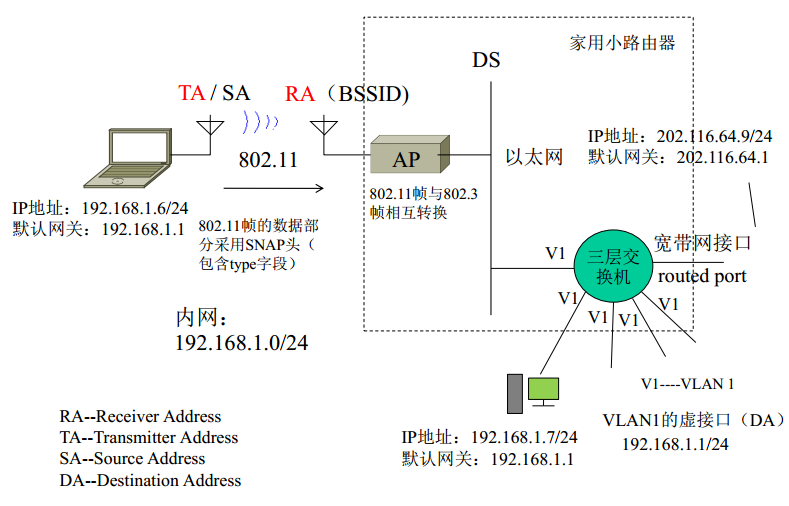
\includegraphics[width=0.8\linewidth]{fig/wlan-example.png}
\end{figure}

\begin{itemize}
\item 很多家用小路由器的内网IP都设成192.168.1.0/24
\item 默认网关配成虚接口的地址(192.168.1.1)
\item 三层交换机的路由表:两个直线网(192.168.1.0/24、202.116.64.9)、默认路由(202.116.64.1),访问因特网就会匹配上默认路由(有线方式)
\item 无线方式:发出来有三个地址
\begin{itemize}
    \item TA(左侧电脑无线网卡的MAC地址)作为SA(源地址)
    \item DA(虚接口的MAC地址)作为目的地址
    \item RA(AP的MAC地址/BSSID),因为有很多个AP,所以要指定RA
\end{itemize}
AP收下帧后,把802.11的帧转化为以太网的帧(有源地址和目的地址了,同时SNAP中也给出了类型),然后用以太网协议发送,三层交换机收到(虚接口地址),再查路由表转发给对应主机或访问外网
\item 当然DA也可以直接写目的主机的IP地址,这样的话交换机就作为透明网桥使用
\end{itemize}

\subsubsection{其他技术}
\begin{itemize}
\item 翻译网桥:一种帧转换为另一种帧
\item 不同频率的WiFi:5GHz WiFi干扰小(不是说现在的5G)
\item 跟以太网不同,WiFi在物理层是有格式的,远距离会换编码,降速进行传输
\item MIMO技术:多发射天线和多接收天线形成多个空间数据流
\end{itemize}

\subsection{网络管理}
SNMP协议:Simple Network Management Protocol

\subsection{广域网}
ADSL不是用语音传,是用数据传的,现在都不用电话线连了。

\subsection{软件定义网络}
软件定义网络(Software Defined Network, SDN):原来路由器交换机都是固定电路,但现在可编程,是未来网络发展方向,最大的好处在于\textemph{虚拟化}。

\begin{center}
\begin{tikzcd}
\text{应用}\arrow{d}\\
\text{控制器}\arrow{d}\\
\text{转发器}
\end{tikzcd}
\end{center}

控制器相当于一个电脑,用来修改下面(几十台)转发器的路由表。

\subsection{多媒体网络}
\begin{itemize}
\item 插值解决丢包问题,因为是连续变化的
\item 传语音数据是用RTP协议传的,基于UDP协议
\item SIP协议用来做网络会议
\item H.232协议则更加完整
\item 令牌桶:没传的时候放令牌,有传的时候用光令牌
\item MPLS加标签实现VPN,沿着同一条路径走过去
\end{itemize}
% !TEX root = main.tex

\section{总结}
\begin{figure}[H]
    \centering
    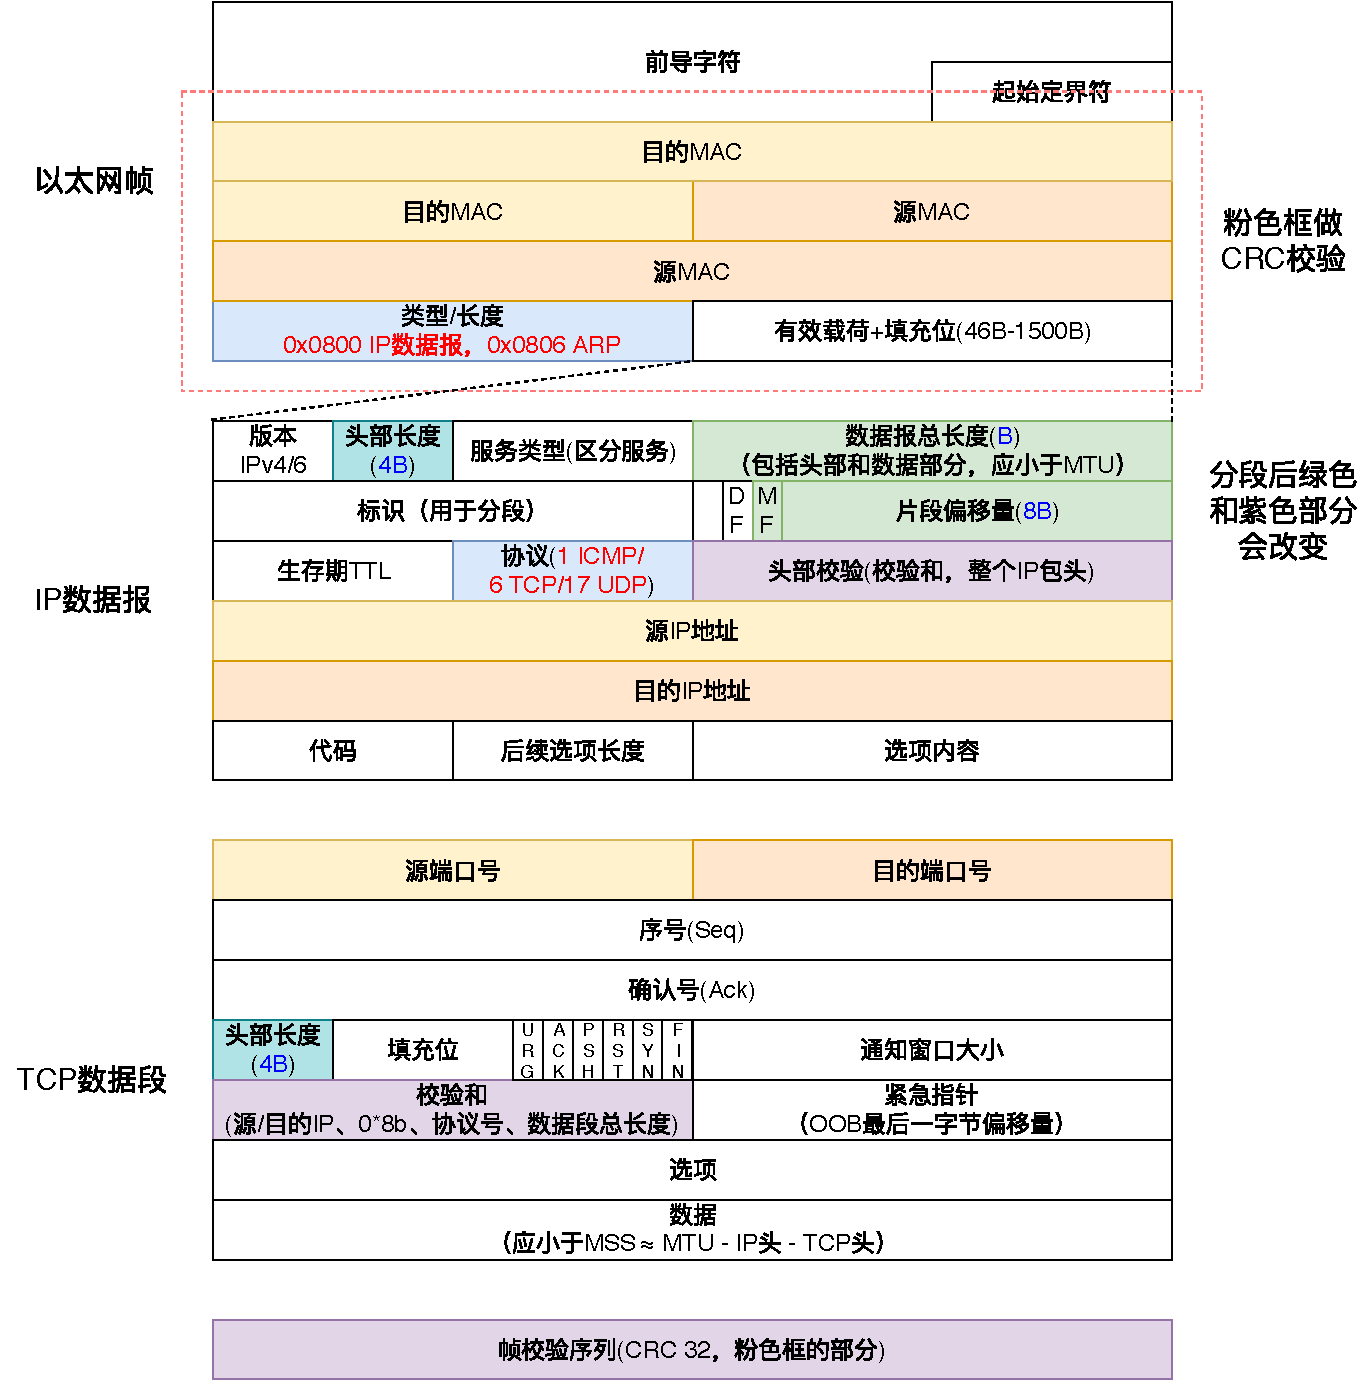
\includegraphics[width=0.9\linewidth]{fig/network-headers.pdf}
\end{figure}

\section{参考资料}
\begin{enumerate}
\item 计算机网络总结,\url{https://blog.csdn.net/n1neding/article/list/7?t=1&}
\end{enumerate}

\end{document}